\chapter{System-level Design}
\label{chap:system-level-design}

\section{Product architecture}

\begin{figure}
  \centering
  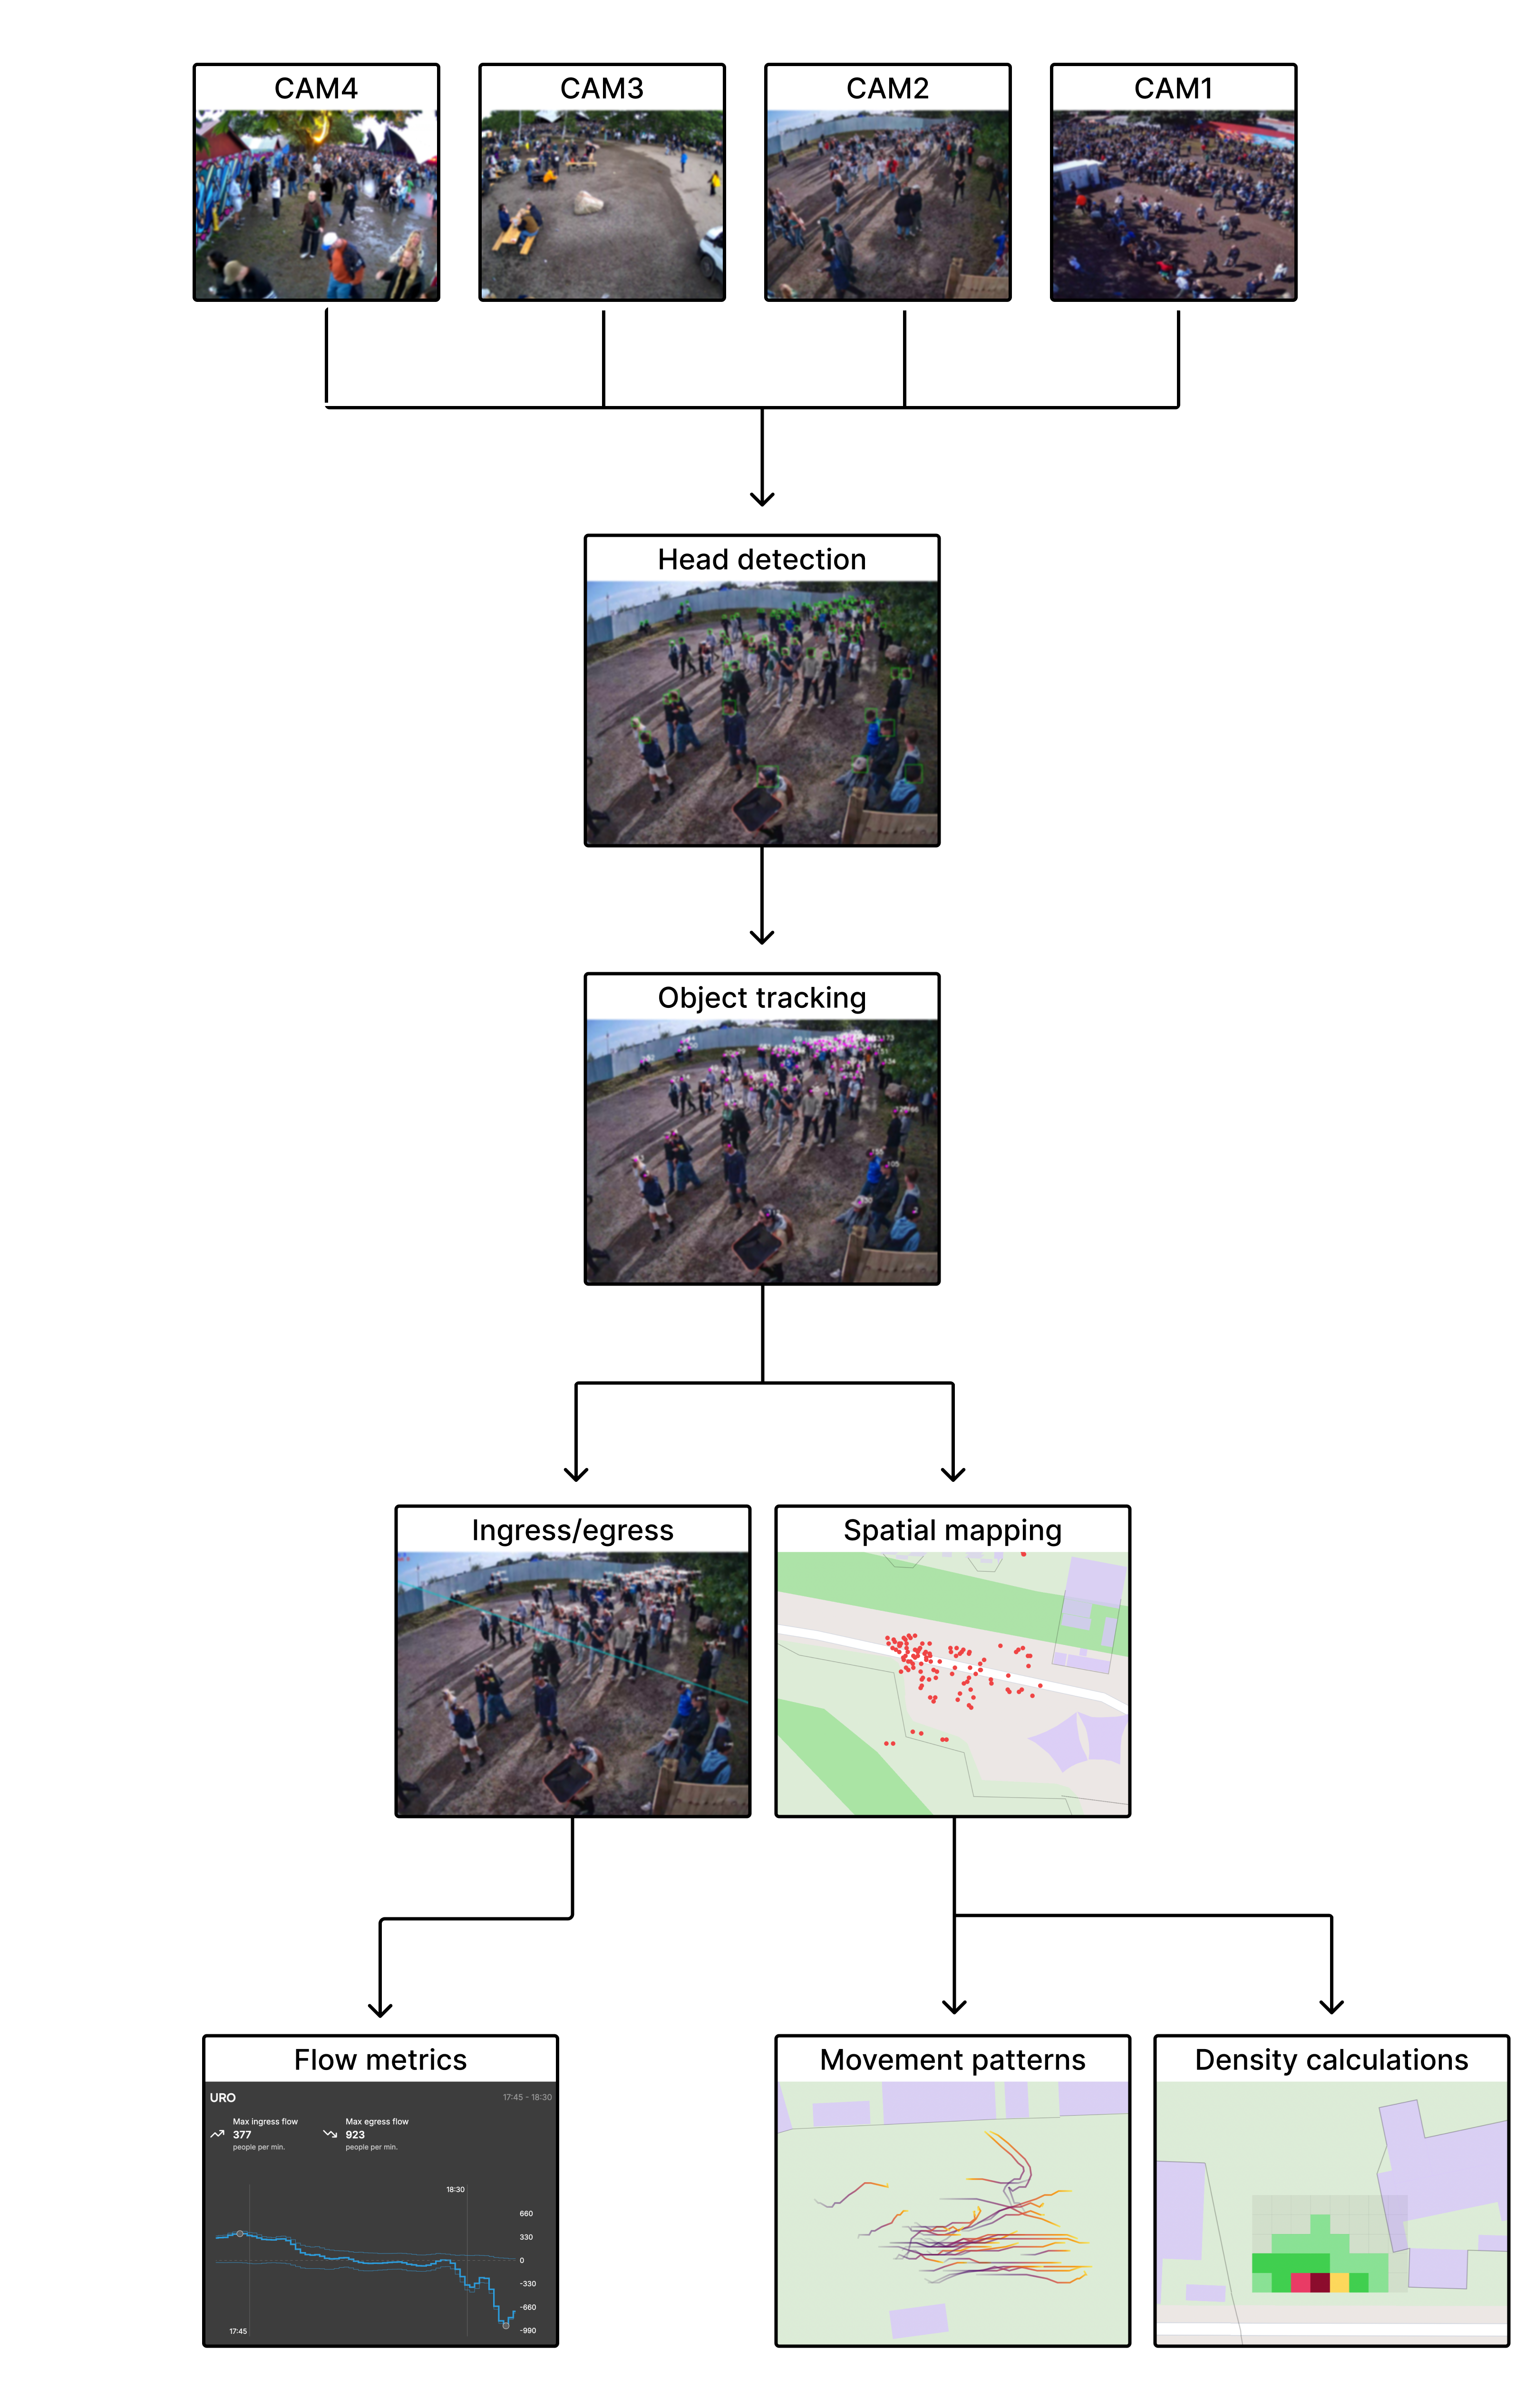
\includegraphics[width=0.9\textwidth]{Pictures/Figures/system_flowchart.png}
  \caption{Flowchart visualizing the system architecture. \textit{Images have been intentionally blurred to protect privacy}.}
\end{figure}


\section{Sub-systems}

\subsection{Data collection}
\label{sec:data_collection}

Data collection constitutes the initial, vital stage of the system, providing the raw data required for all subsequent processing and analysis. This process entailed the on-site deployment of designated cameras, strategically positioned to capture the targeted crowd dynamics.

The selected cameras were Reolink RLC-520A, which are PoE-enabled (Power over Ethernet) and capable of recording 5MP (2560x1920 pixels) video at 30 frames per second. A separate PoE switch (Ubiquiti PoE++ Adapter), connected to a standard power outlet, was required to power the cameras. This setup allowed connection to the cameras via an Ethernet cable linked to a laptop, enabling camera configuration and live feed monitoring. Utilizing the cameras' integrated software, recording windows could be predefined such that footage would automatically be archived on the internal SD card. This setup was designed to ensure that the cameras could operate independently without requiring a constant connection to a computer. Mounting the cameras was achieved with 3D-printed brackets, designed to securely attach the cameras to existing infrastructure, such as fences or poles. Where existing structures were unavailable, aluminum poles were utilized to achieve the necessary height for capturing the entire designated area. Four cameras were deployed, denoted as \textit{CAM1}, \textit{CAM2}, \textit{CAM3}, and \textit{CAM4}.

As agreed upon with Roskilde Festival's safety team, the cameras were installed around the Eos stage during the first three days of the festival, and subsequently moved to the Arena stage for the remainder of the festival.

Determining camera placement for the Eos stage was relatively trivial. During the festival's "First Days," (June 30th to July 2nd) the remainder of the festival site, excluding the Gaia stage, was closed off to guests, leaving only two pathways for entering and exiting the stage area. At each of these two pathways, two cameras were installed, oriented to face one another. \textit{CAM1} and \textit{CAM3} were positioned at Eos' southern entrance, Entrance 10, while \textit{CAM2} and \textit{CAM4} were placed at the eastern entrance, towards the Gaia stage (Figure \ref{fig:eos_cameras}). This dual-camera configuration served two purposes: ensuring complete monitoring of the pathway's width, as well as providing a redundant dataset for each location, effectively mitigating the risk of equipment malfunction during the initial deployment.

\begin{figure}
  \centering
  \begin{subfigure}{0.9\textwidth}
    \centering
    \includegraphics[width=\textwidth]{Pictures/Figures/eos_cameras.png}
    \caption{Eos stage area -- visualized with camera placements}
  \end{subfigure}
  \begin{subfigure}{0.42\textwidth}
    \centering
    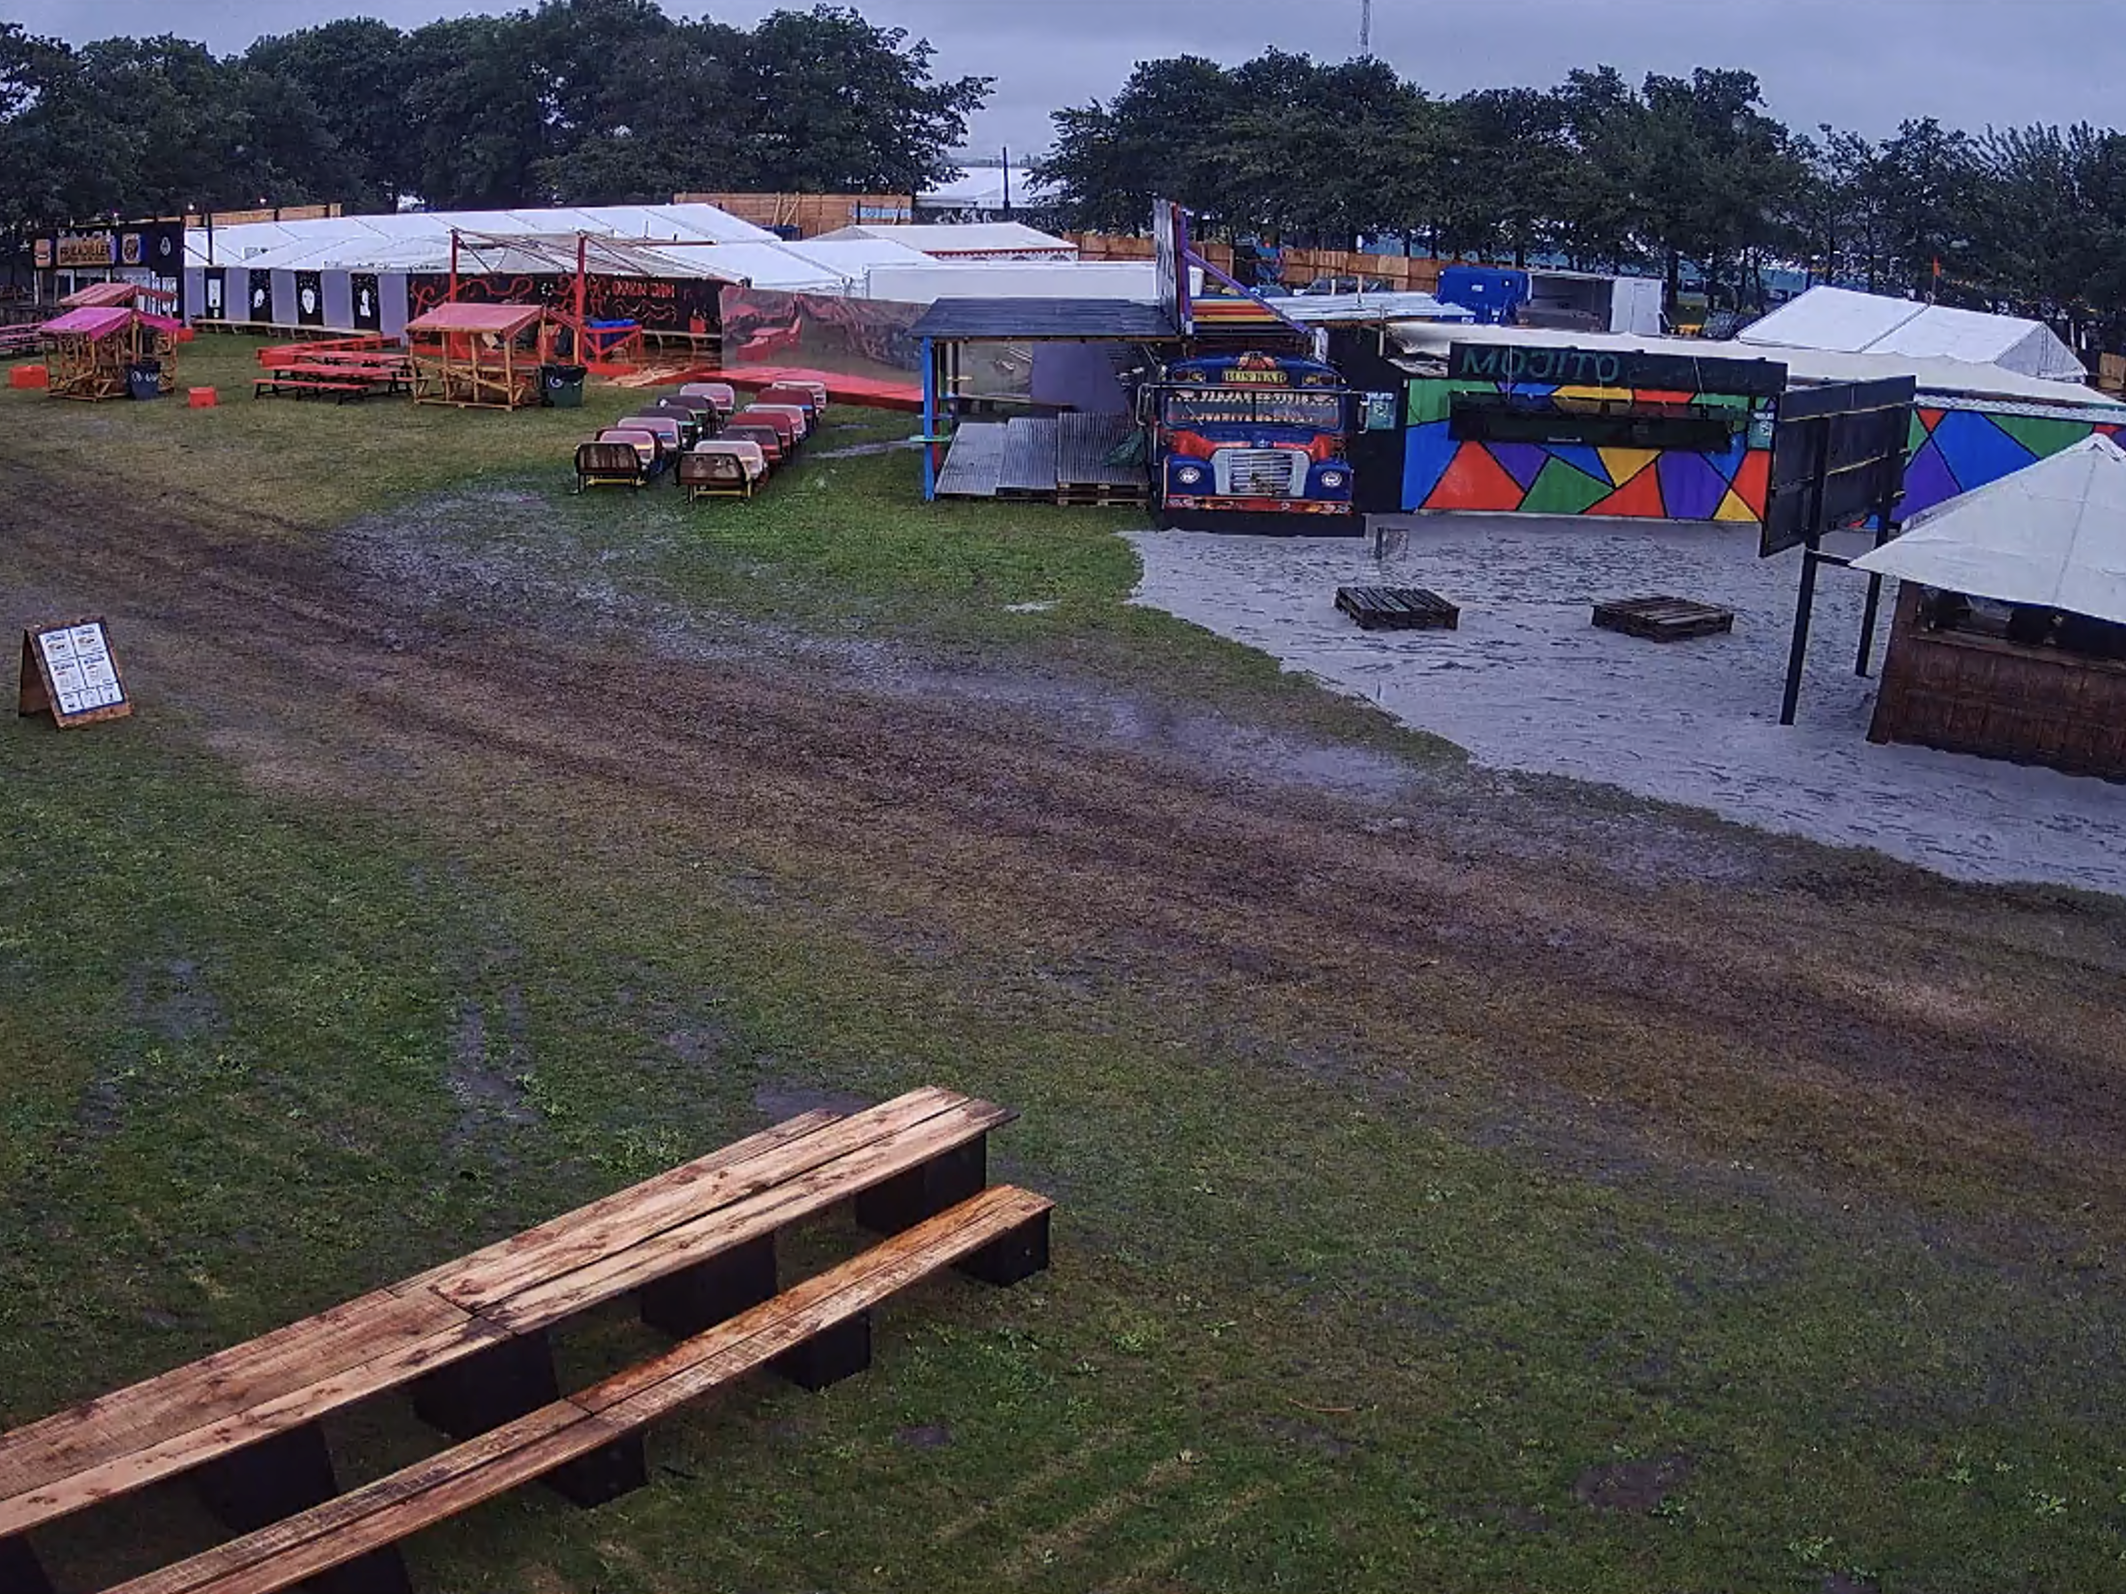
\includegraphics[width=\textwidth]{Pictures/Misc/Cameras/EOS_CAM1.png}
    \caption{CAM1 Preview}
  \end{subfigure}%
  \hspace{0.06\textwidth}
  \begin{subfigure}{0.42\textwidth}
    \centering
    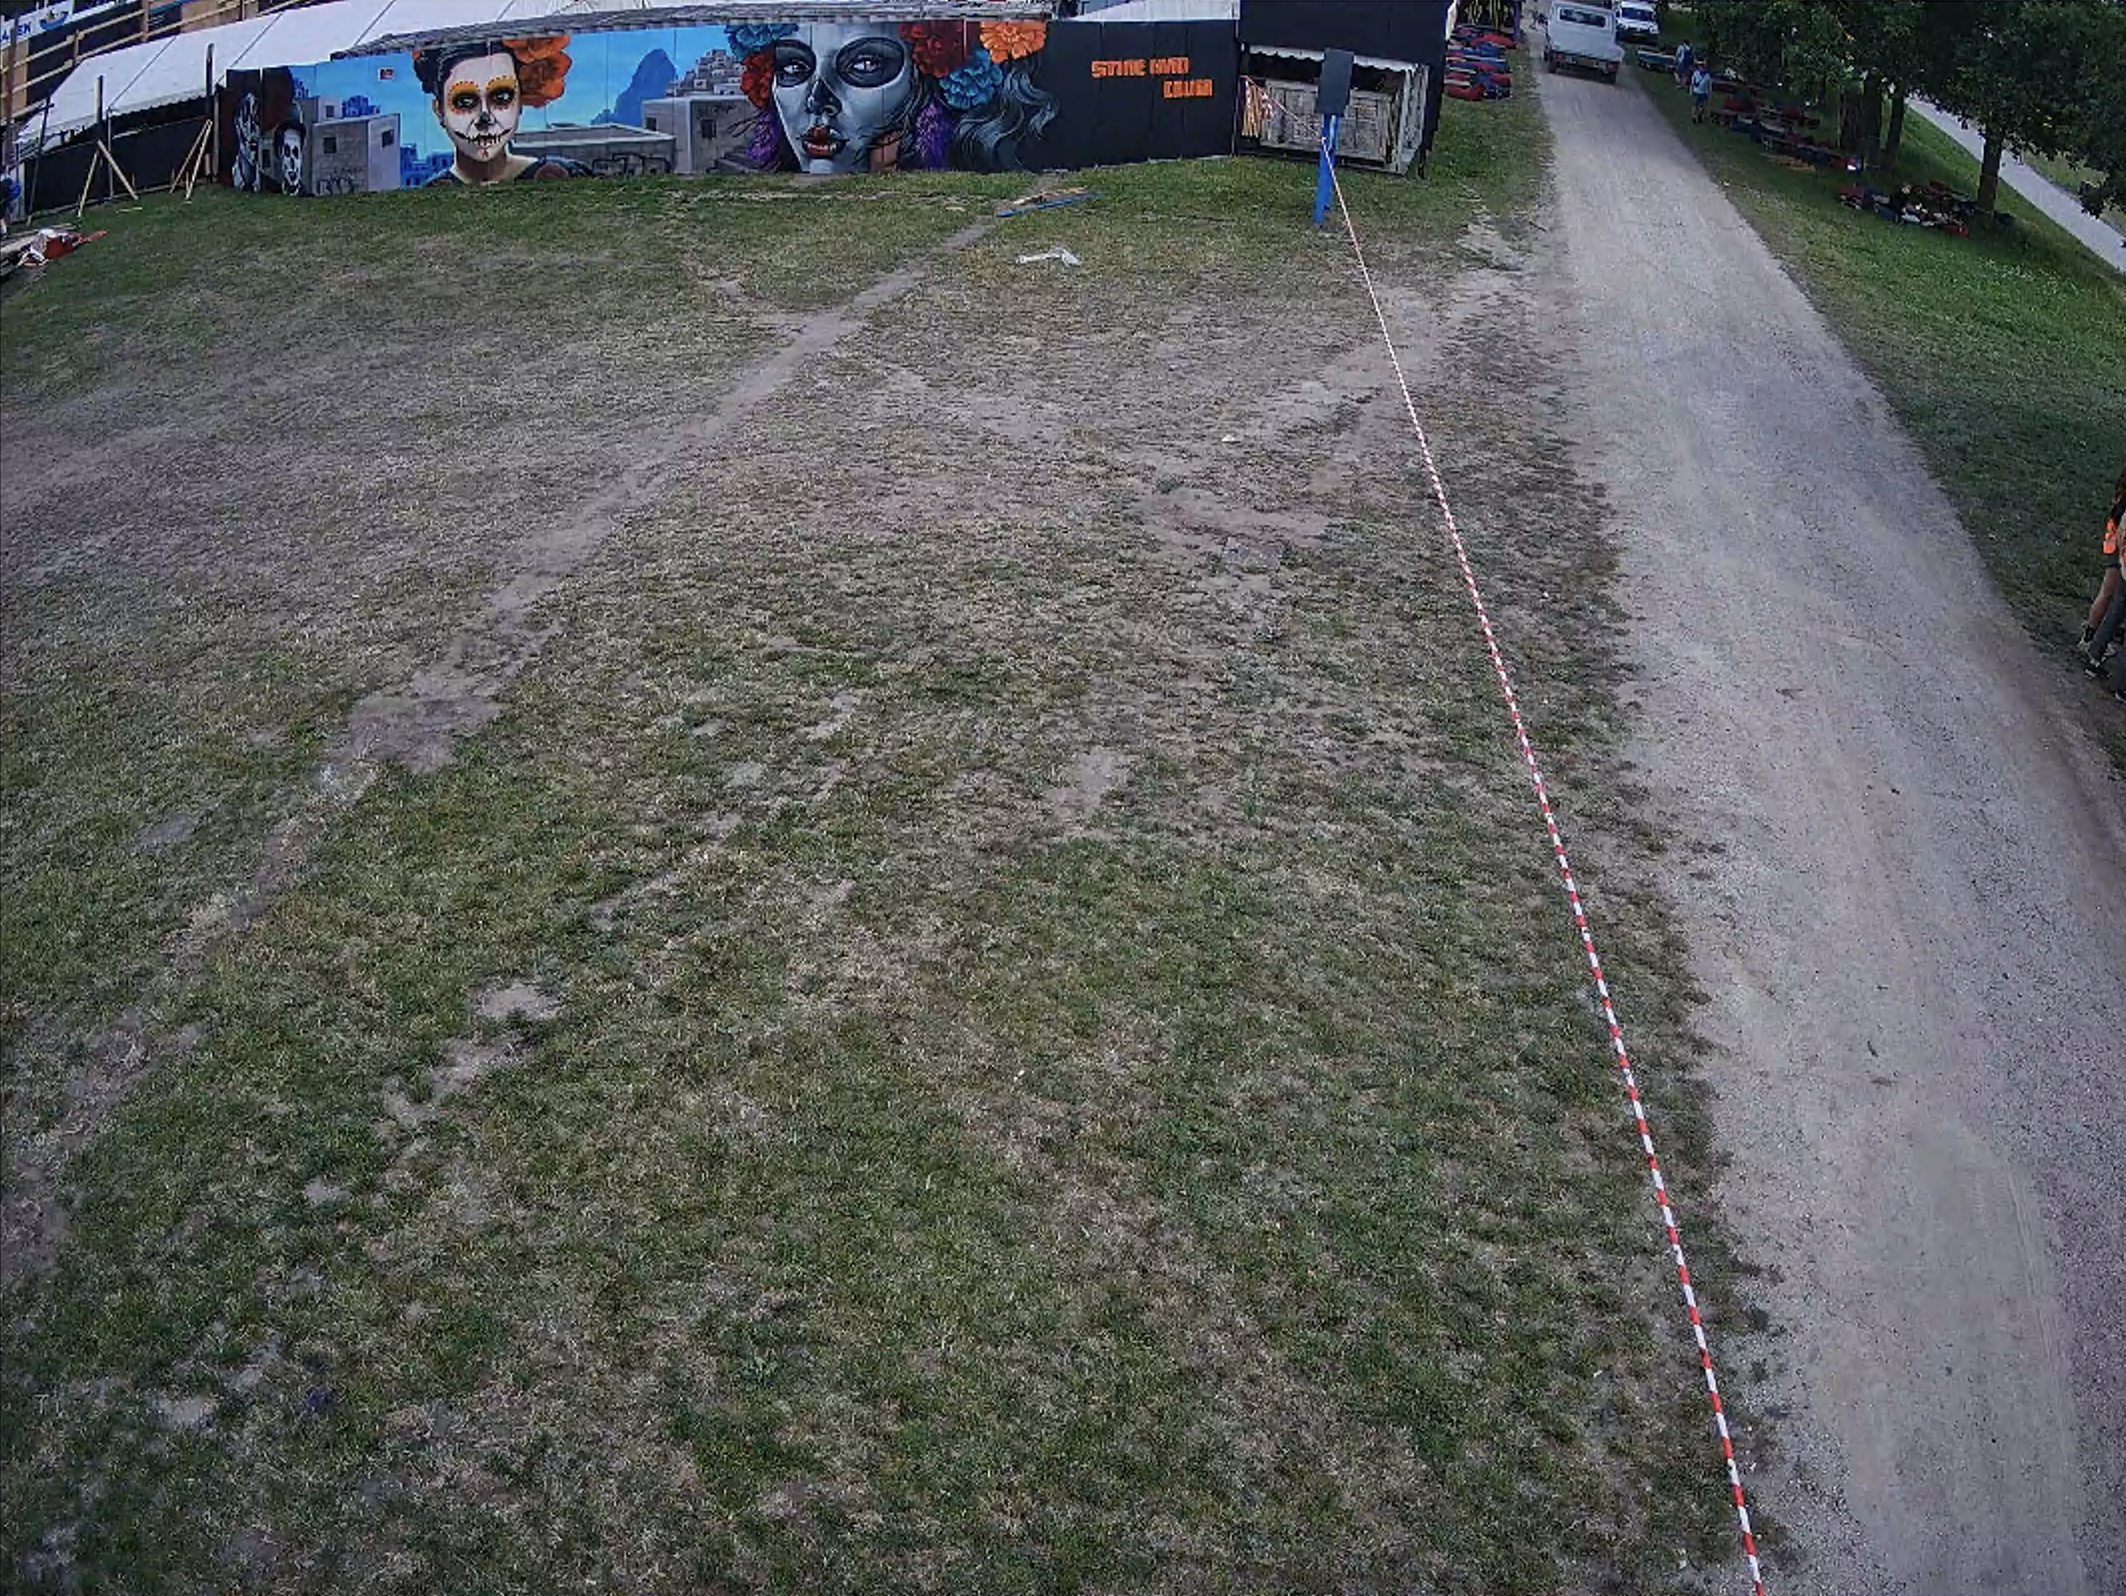
\includegraphics[width=\textwidth]{Pictures/Misc/Cameras/EOS_CAM2.png}
    \caption{CAM2 Preview}
  \end{subfigure}

  \begin{subfigure}{0.42\textwidth}
    \centering
    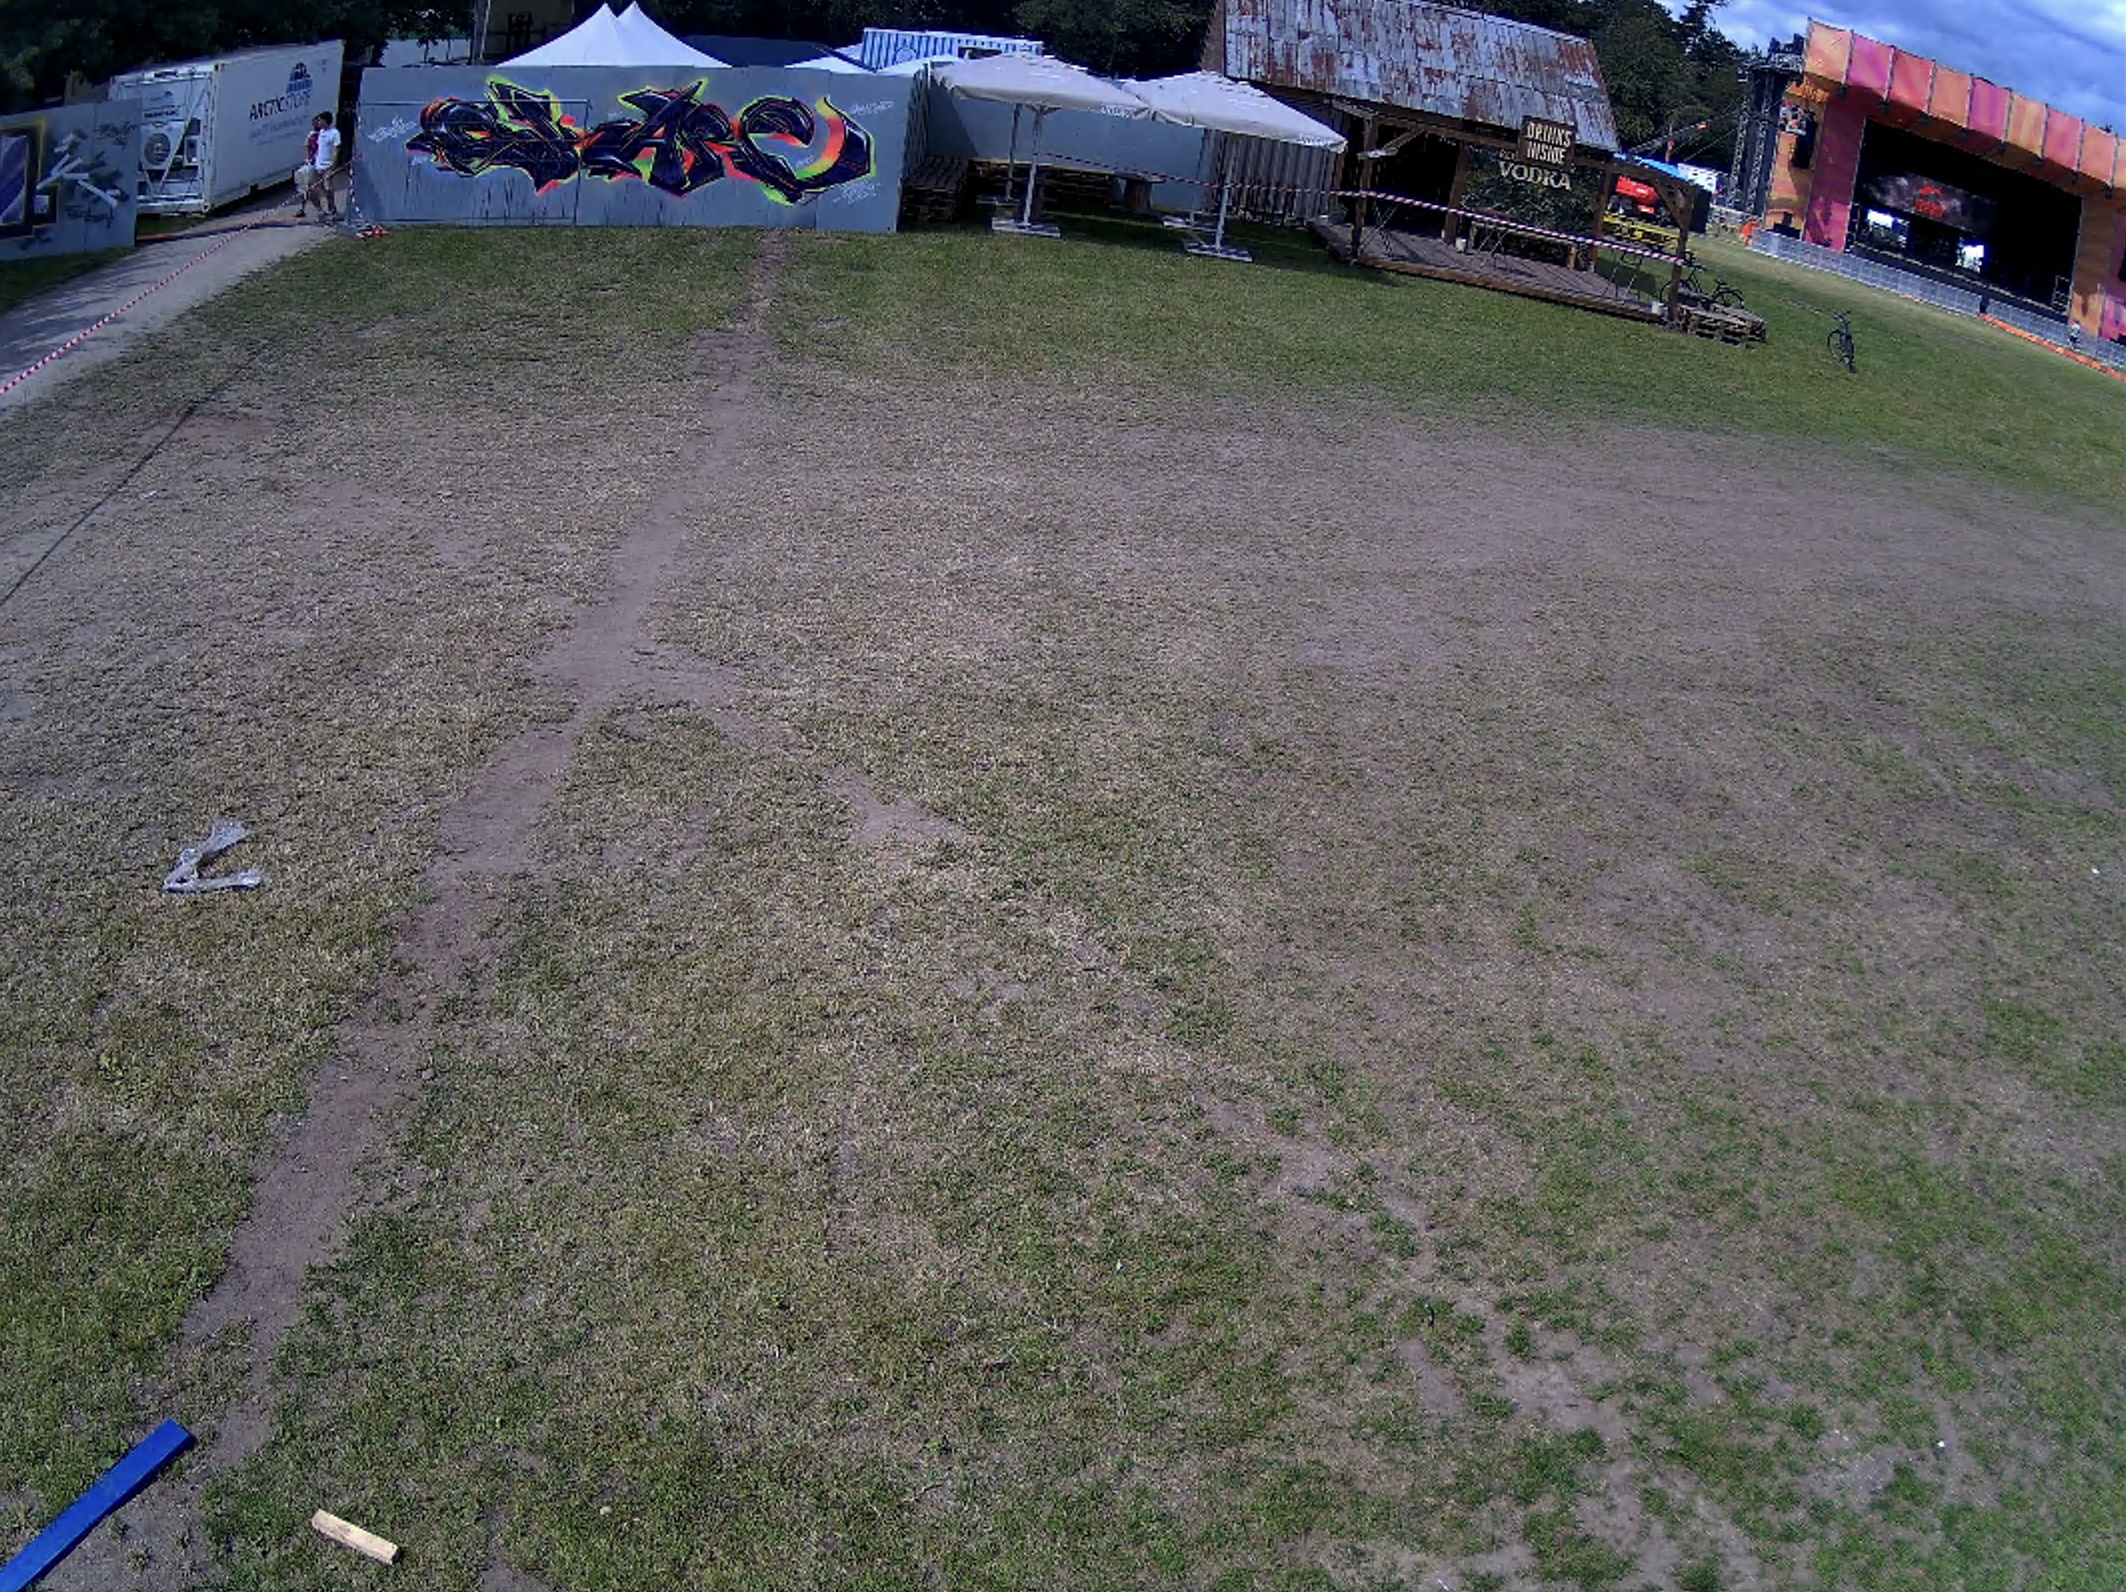
\includegraphics[width=\textwidth]{Pictures/Misc/Cameras/EOS_CAM3.png}
    \caption{CAM3 Preview}
  \end{subfigure}%
  \hspace{0.06\textwidth}
  \begin{subfigure}{0.42\textwidth}
    \centering
    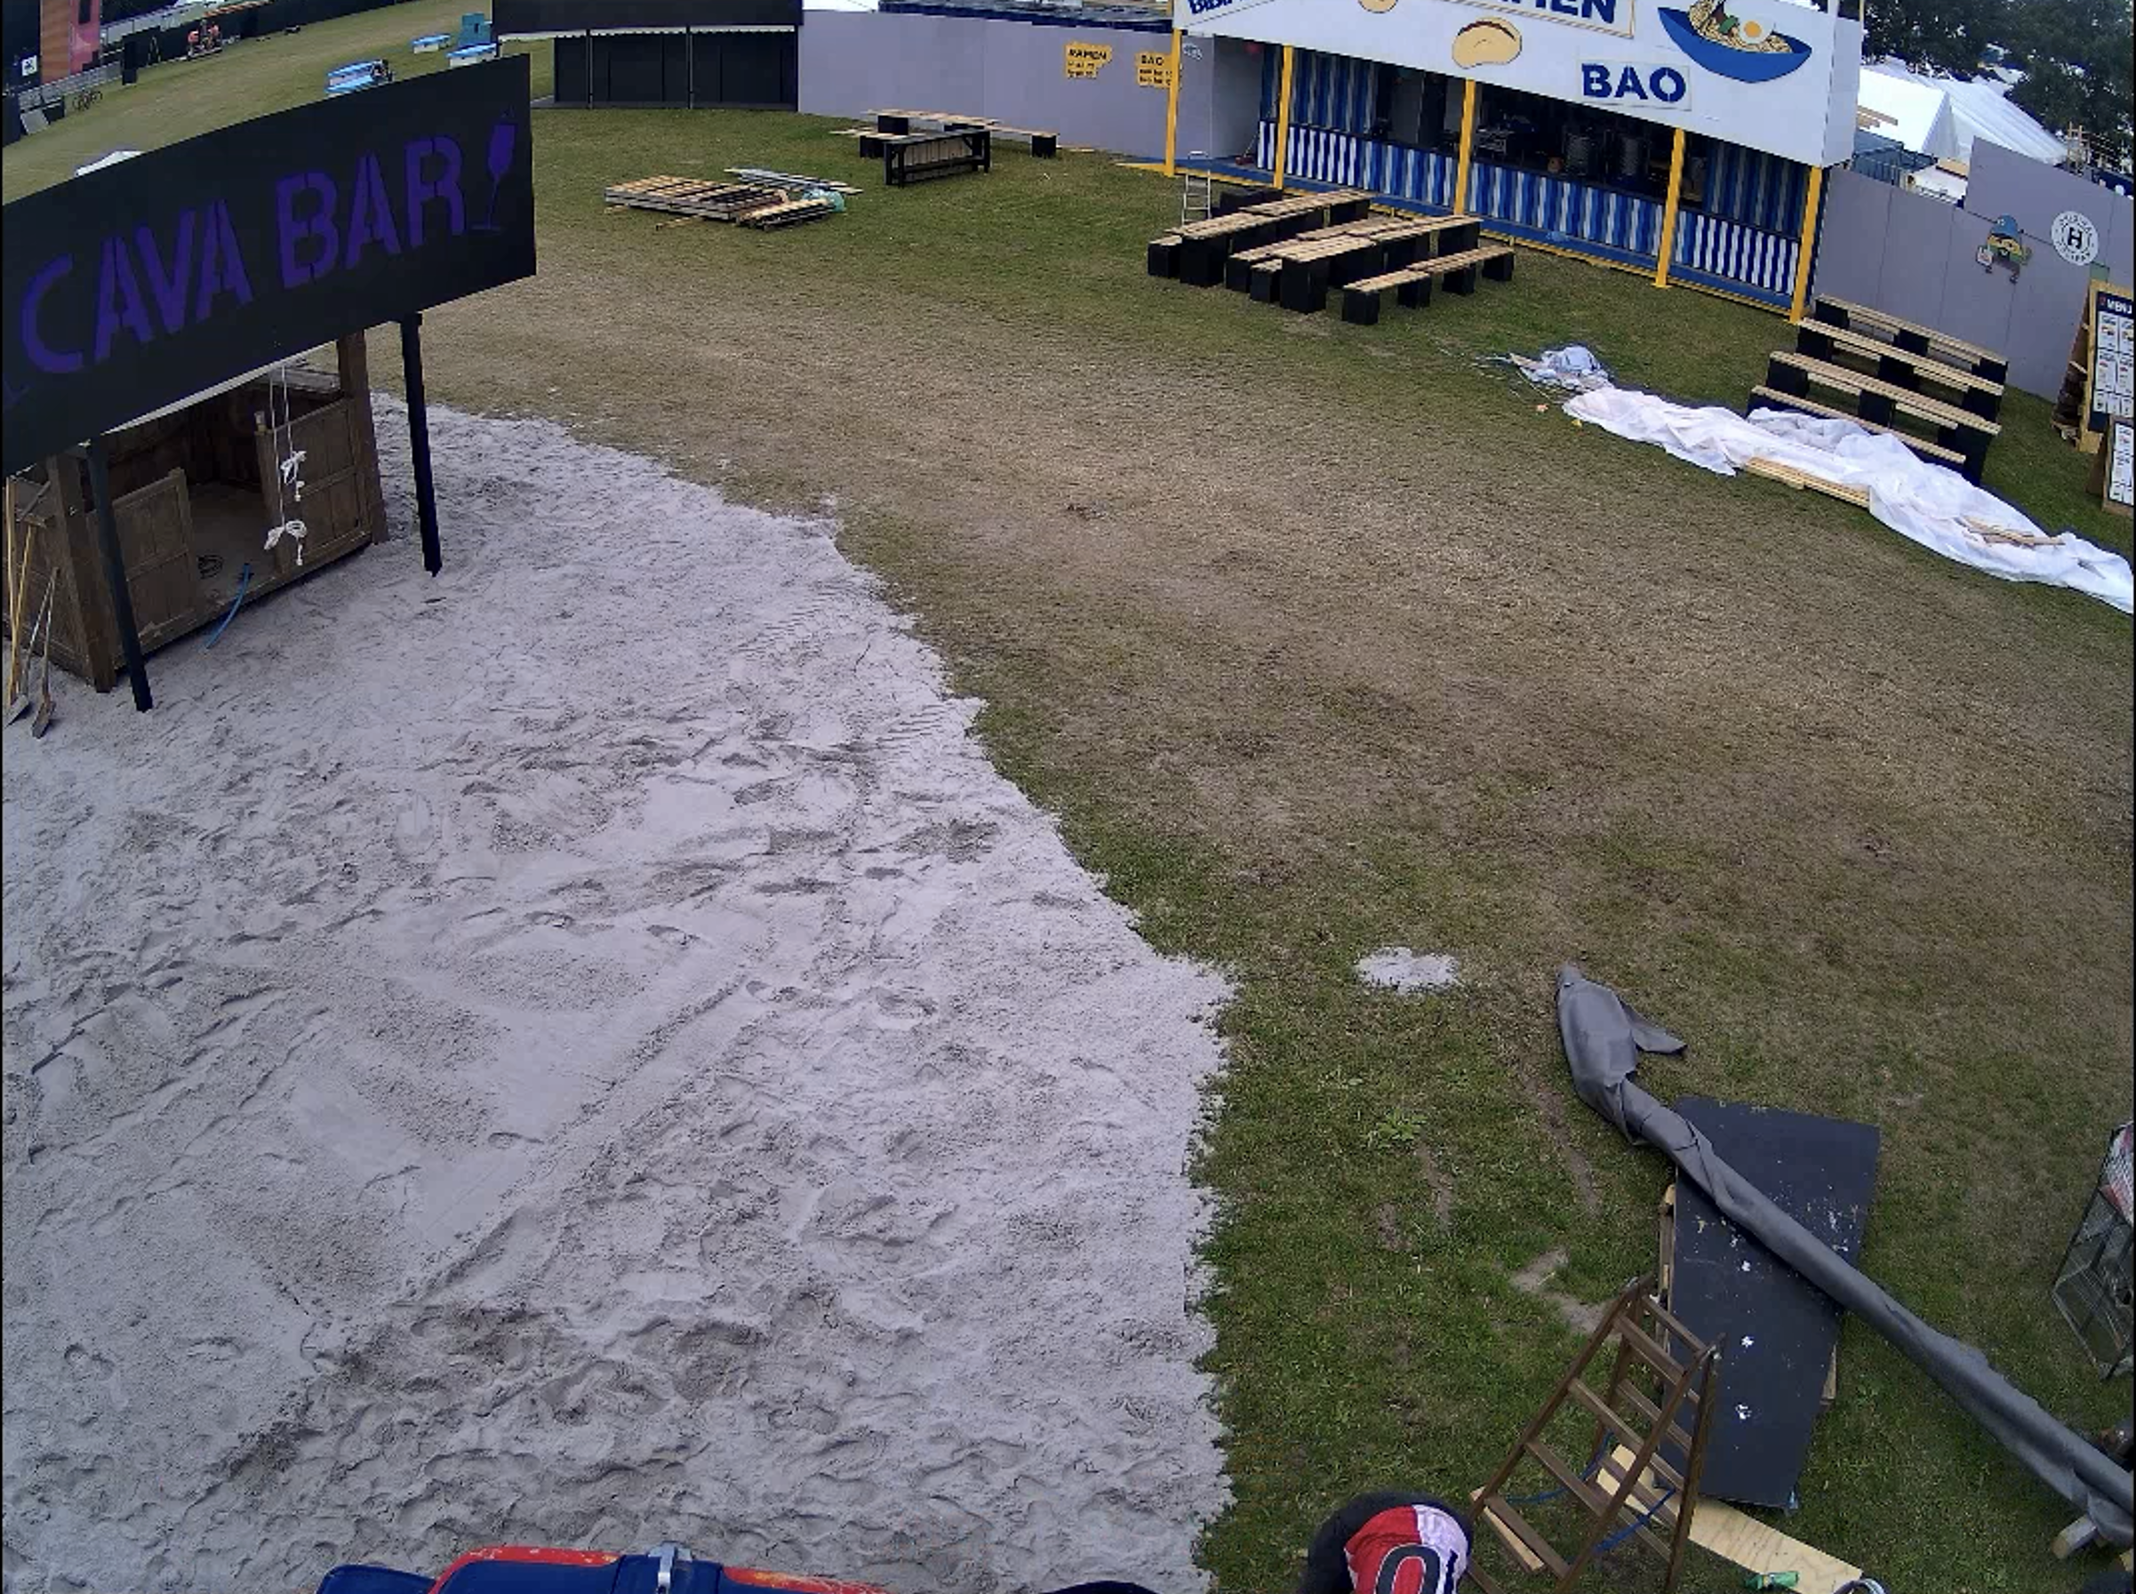
\includegraphics[width=\textwidth]{Pictures/Misc/Cameras/EOS_CAM4.png}
    \caption{CAM4 Preview}
  \end{subfigure}

  \caption{Camera placement at Eos stage, with approximate field of view (FOV) indicated (a). The bottom images show sample frames from the four cameras deployed at the Eos stage, showing the field of view for each camera position (b-e).}
  \label{fig:eos_cameras}

\end{figure}


Camera placement for the Arena stage presented greater complexity due to its significantly larger scale and increased number of entrance and exit points. Arena is located at the far eastern corner of the festival grounds, and it was anticipated that the majority of attendees would approach from the western side, where the remainder of the festival's stages are located. This involved three possible entrances/exits: \textit{the Stables}, \textit{the Graffiti Walk}, and \textit{the Fast-Track}. As the Graffiti Walk is the broadest and most heavily trafficked route, \textit{CAM1} was mounted atop a tall utility pole to ensure comprehensive coverage of this wide pathway. \textit{CAM2} was mounted on an aluminum pole to overlook the fast-track, and \textit{CAM4} was positioned to capture the stables entrance. Finally, \textit{CAM3} was placed at the southeast corner of the stage, at a junction point of the fast-track and Entrances 5 \& 6. This camera was positioned to capture individuals entering and exiting the latter two pathways. Altogether, these camera positions were designed to theoretically provide full coverage of the Arena stage's entrances and exits, allowing accurate metric extraction (Section \ref{sec:metric_extraction}). See Figure \ref{fig:arena_cameras} for a visualization of the camera placements.

The Reolink RLC-520A cameras also included infrared (IR) night vision capabilities, theoretically allowing for monitoring in low-light conditions. However, this feature proved ineffective in practice as the integrated software lacked functionality for time-based switching between day and night modes, offering only a subjective slider for "ambient brightness". This created unpredictability in terms of when the cameras would switch between modes, sometimes leading to the cameras using IR imaging during daylight hours. As this resulted in reduced image quality and limitations on the video frame rate, the cameras were configured to operate without the IR functionality. Therefore, the cameras were set to record continuously for only 12 hours each day, from 12:00 to 24:00. Furthermore, due to the cameras' maximum SD card storage capacity of 256 GB, archived footage required manual download and purging when relocating the equipment between stages.

\begin{figure}
  \centering
  \begin{subfigure}{0.8\textwidth}
    \centering
    \includegraphics[width=\textwidth]{Pictures/Figures/arena_cameras.png}
    \caption{Arena stage area -- visualized with camera placements}

  \end{subfigure}
  \begin{subfigure}{0.37\textwidth}
    \centering
    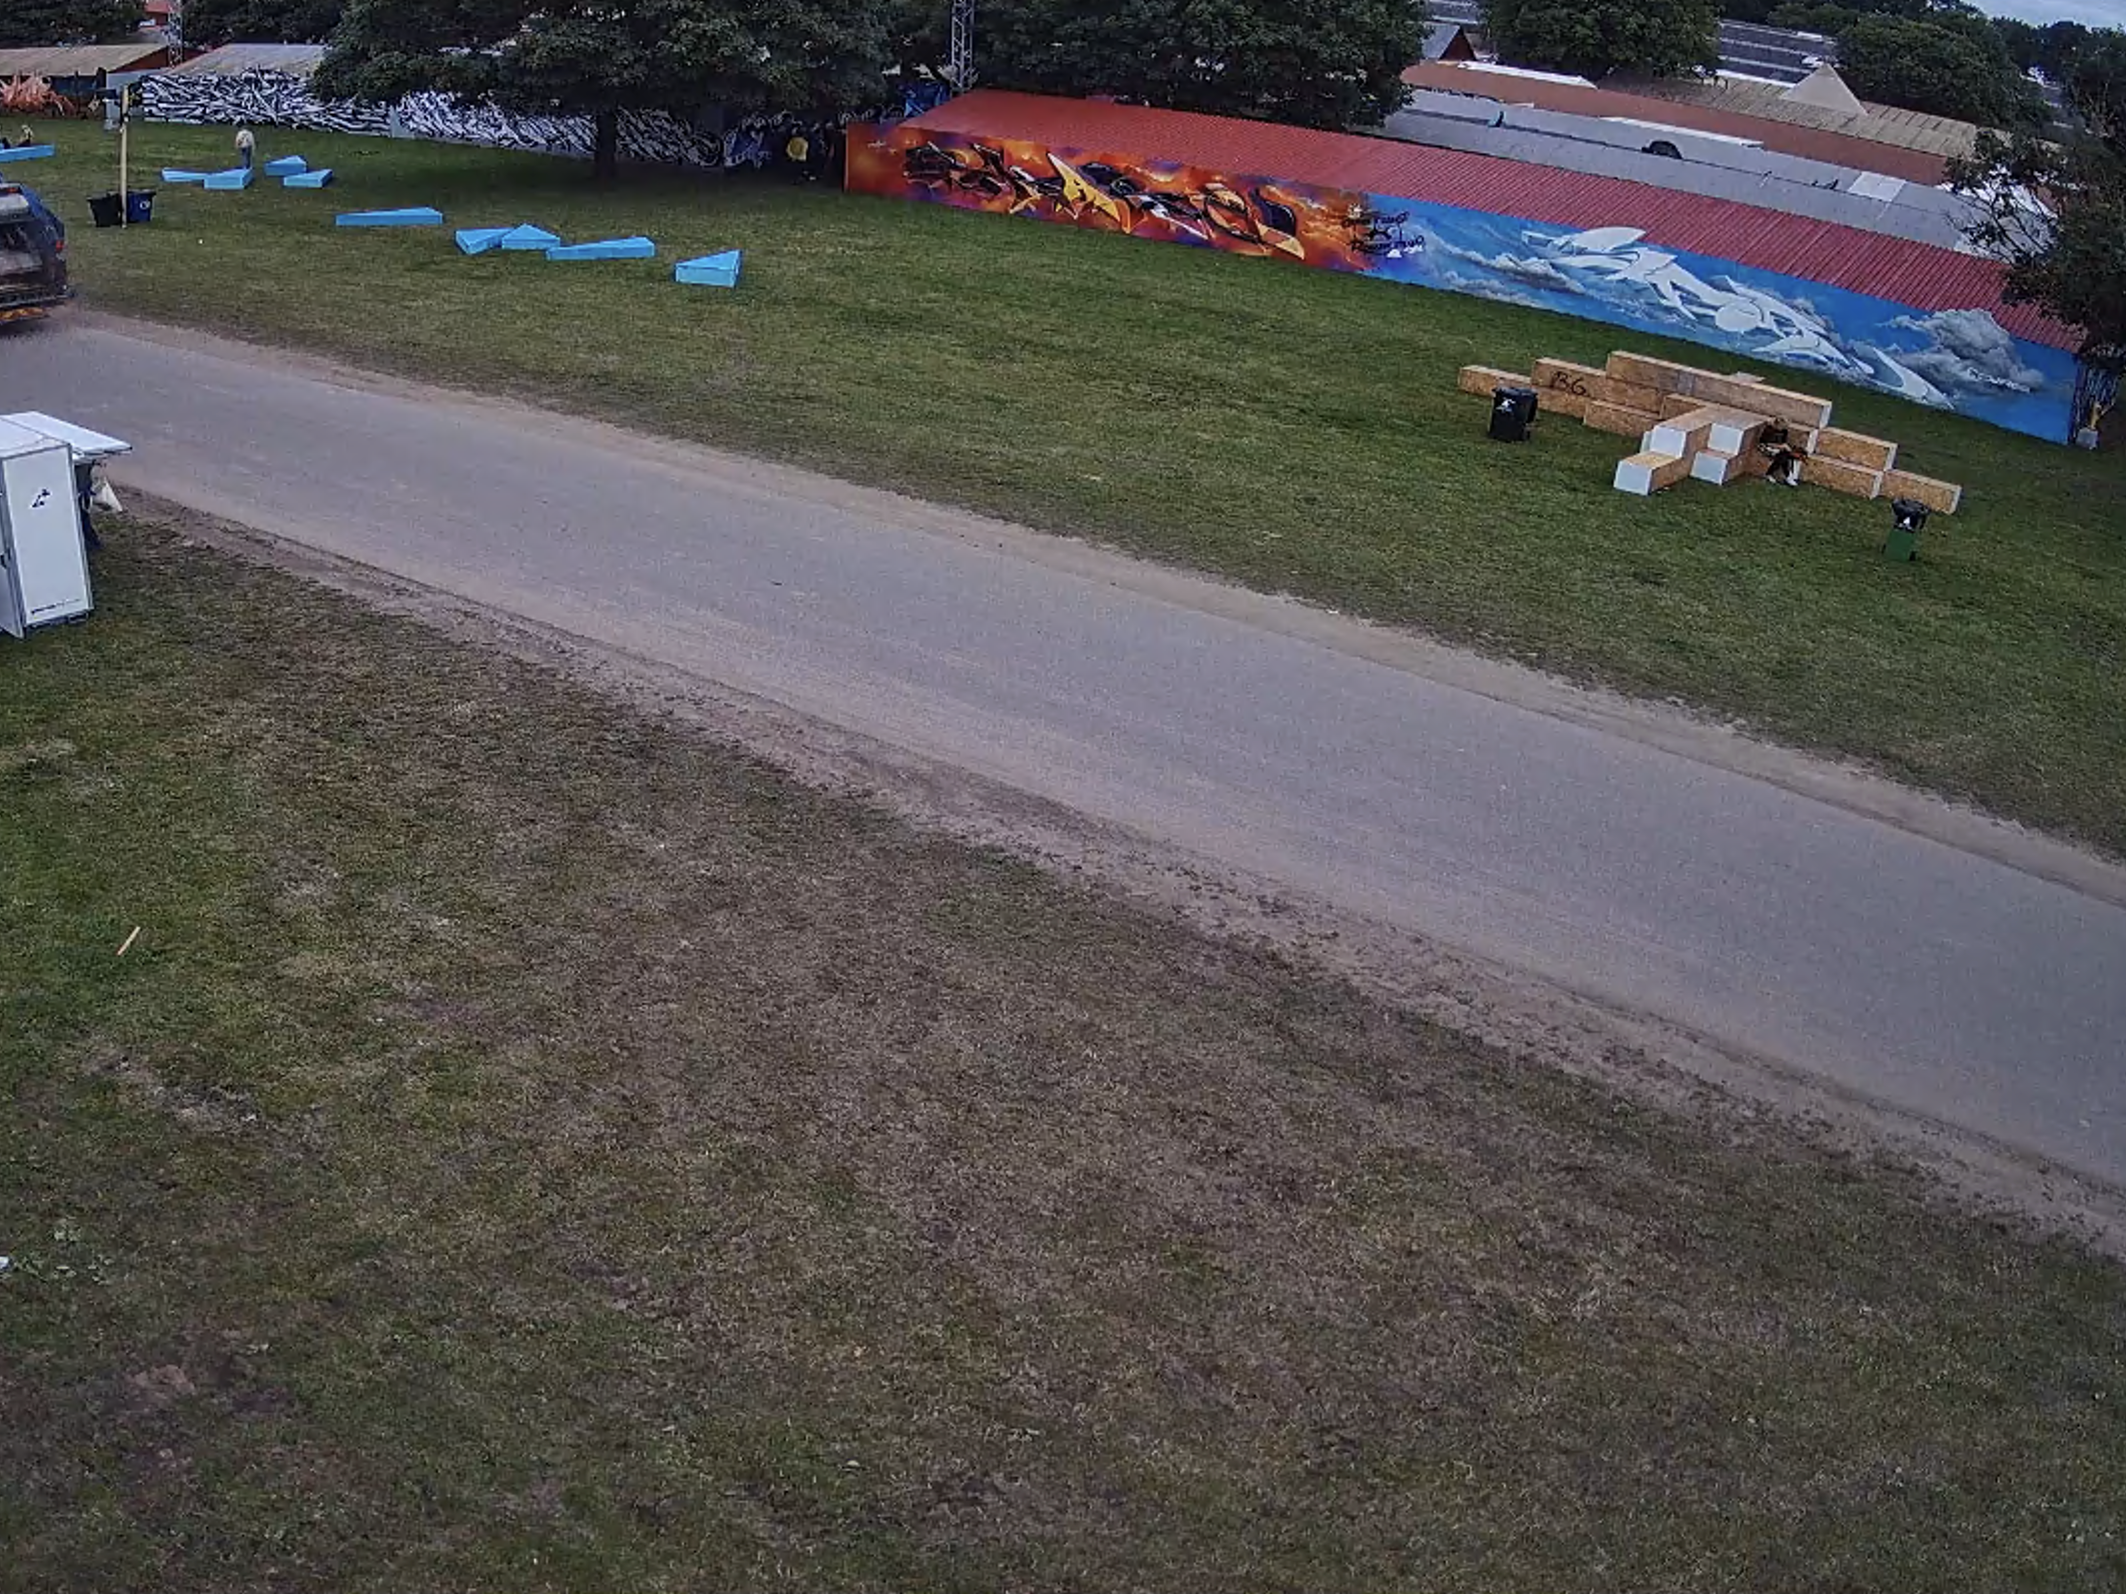
\includegraphics[width=\textwidth]{Pictures/Misc/Cameras/ARENA_CAM1.png}
    \caption{CAM1 Preview}
  \end{subfigure}%
  \hspace{0.06\textwidth}
  \begin{subfigure}{0.37\textwidth}
    \centering
    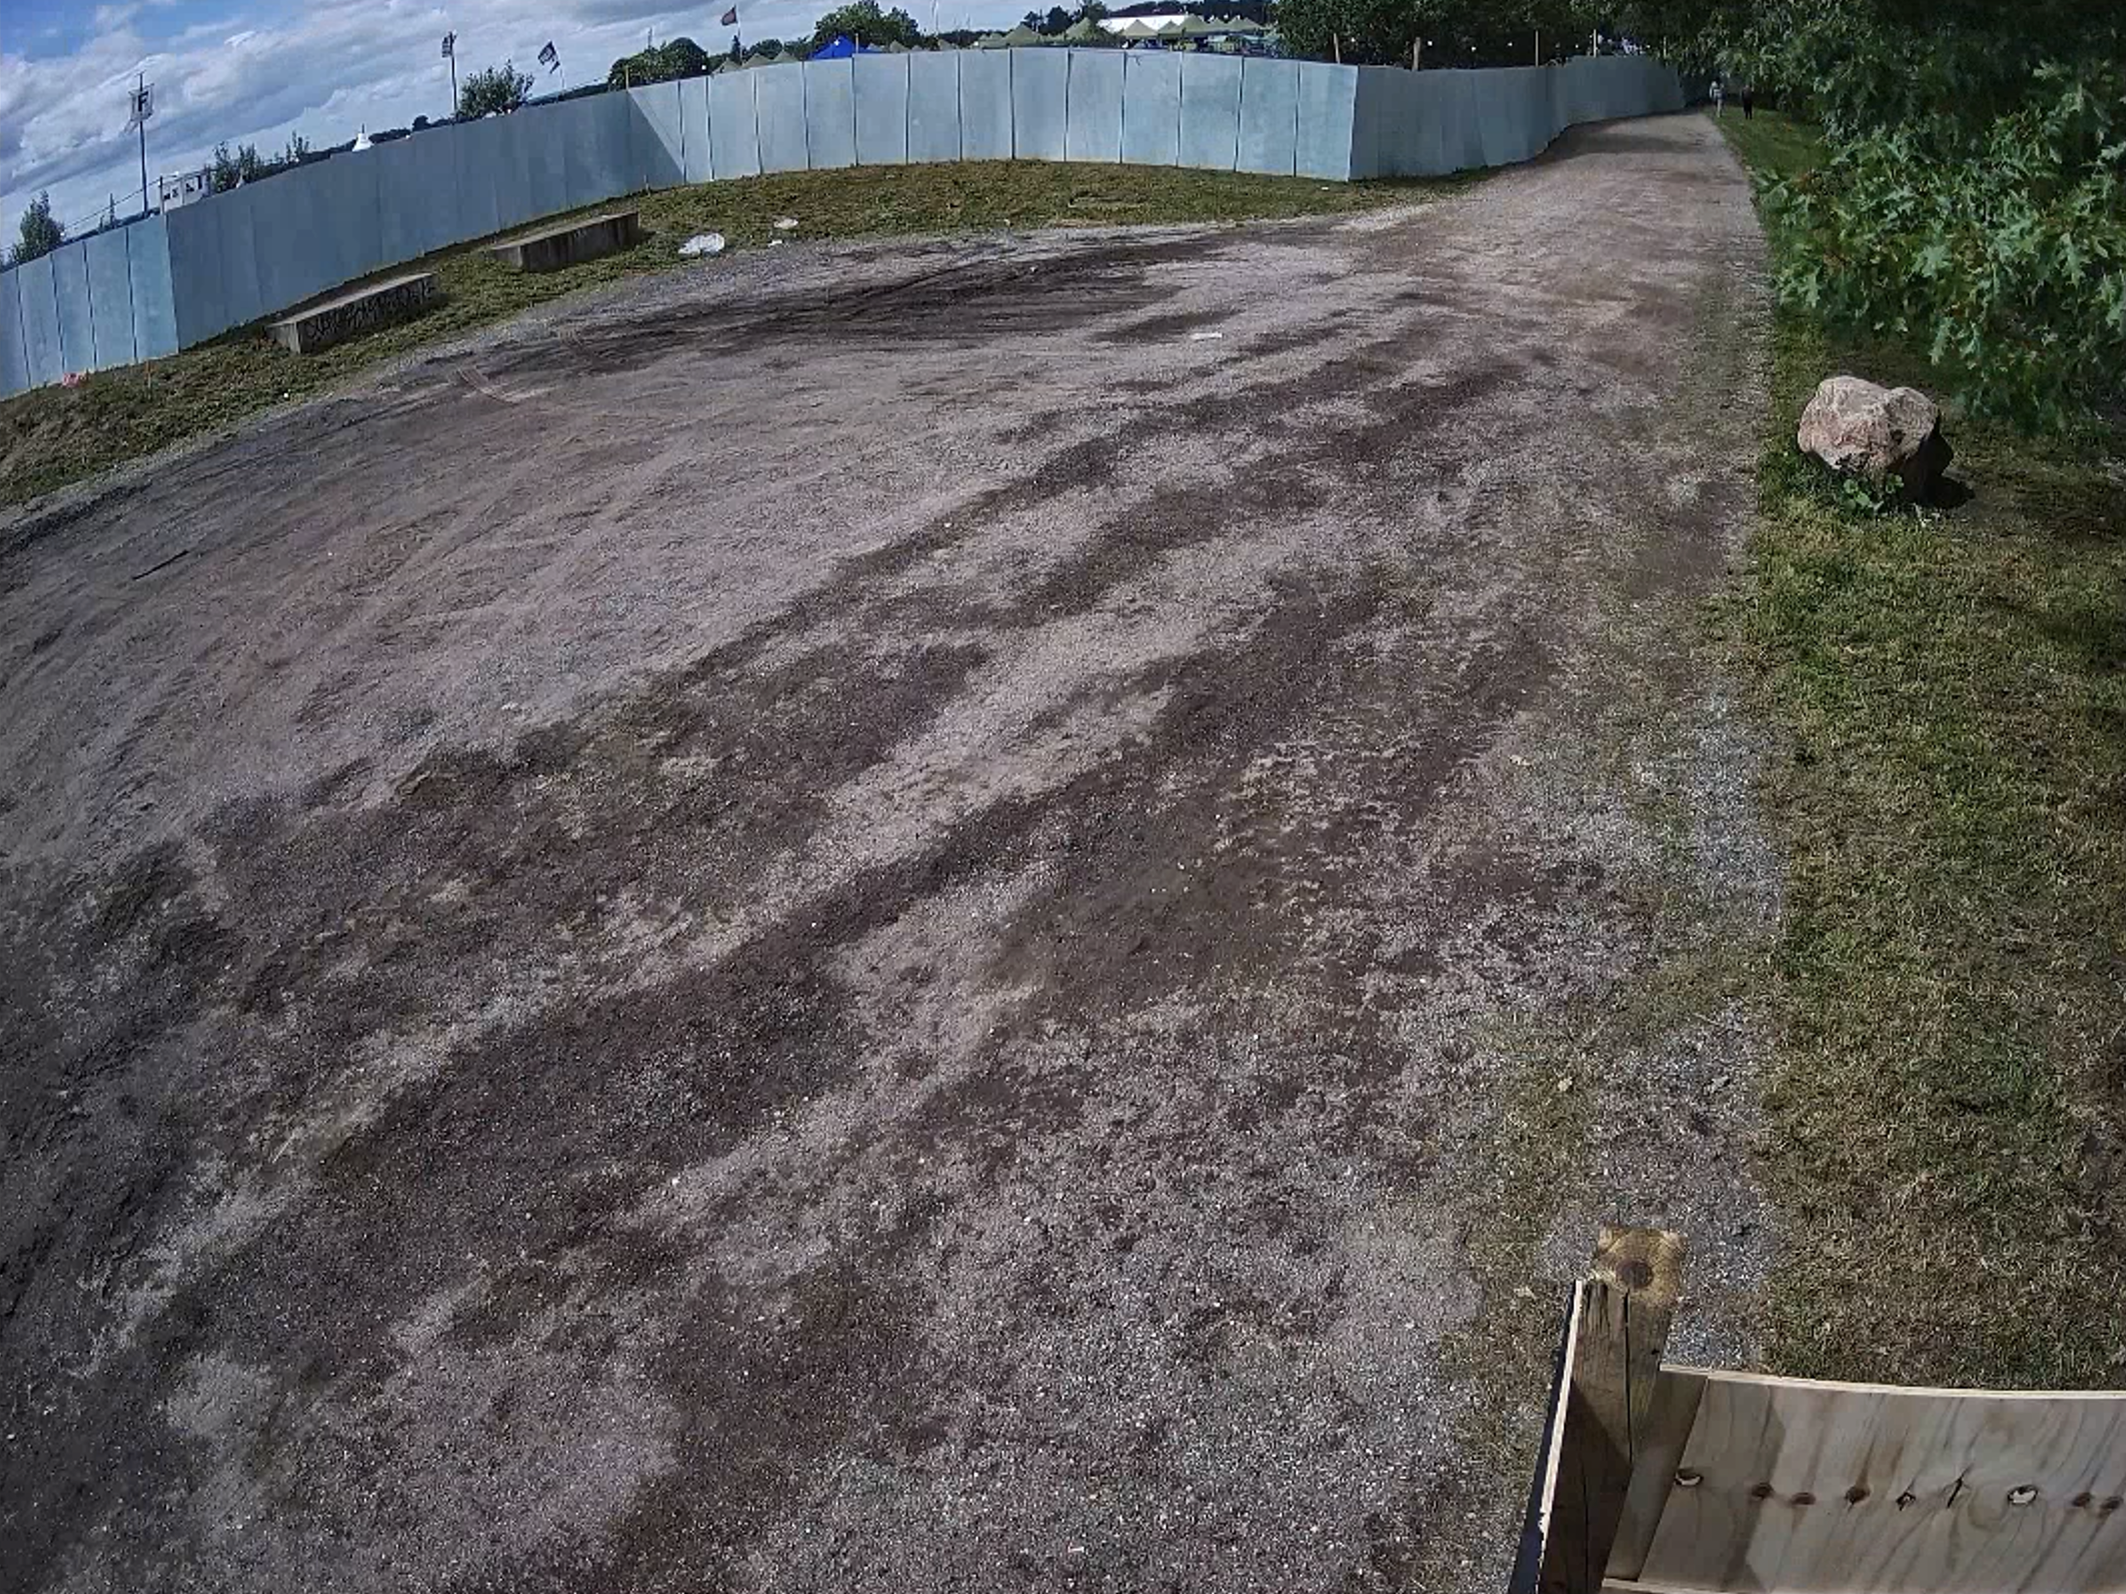
\includegraphics[width=\textwidth]{Pictures/Misc/Cameras/ARENA_CAM2.png}
    \caption{CAM2 Preview}
  \end{subfigure}

  \begin{subfigure}{0.37\textwidth}
    \centering
    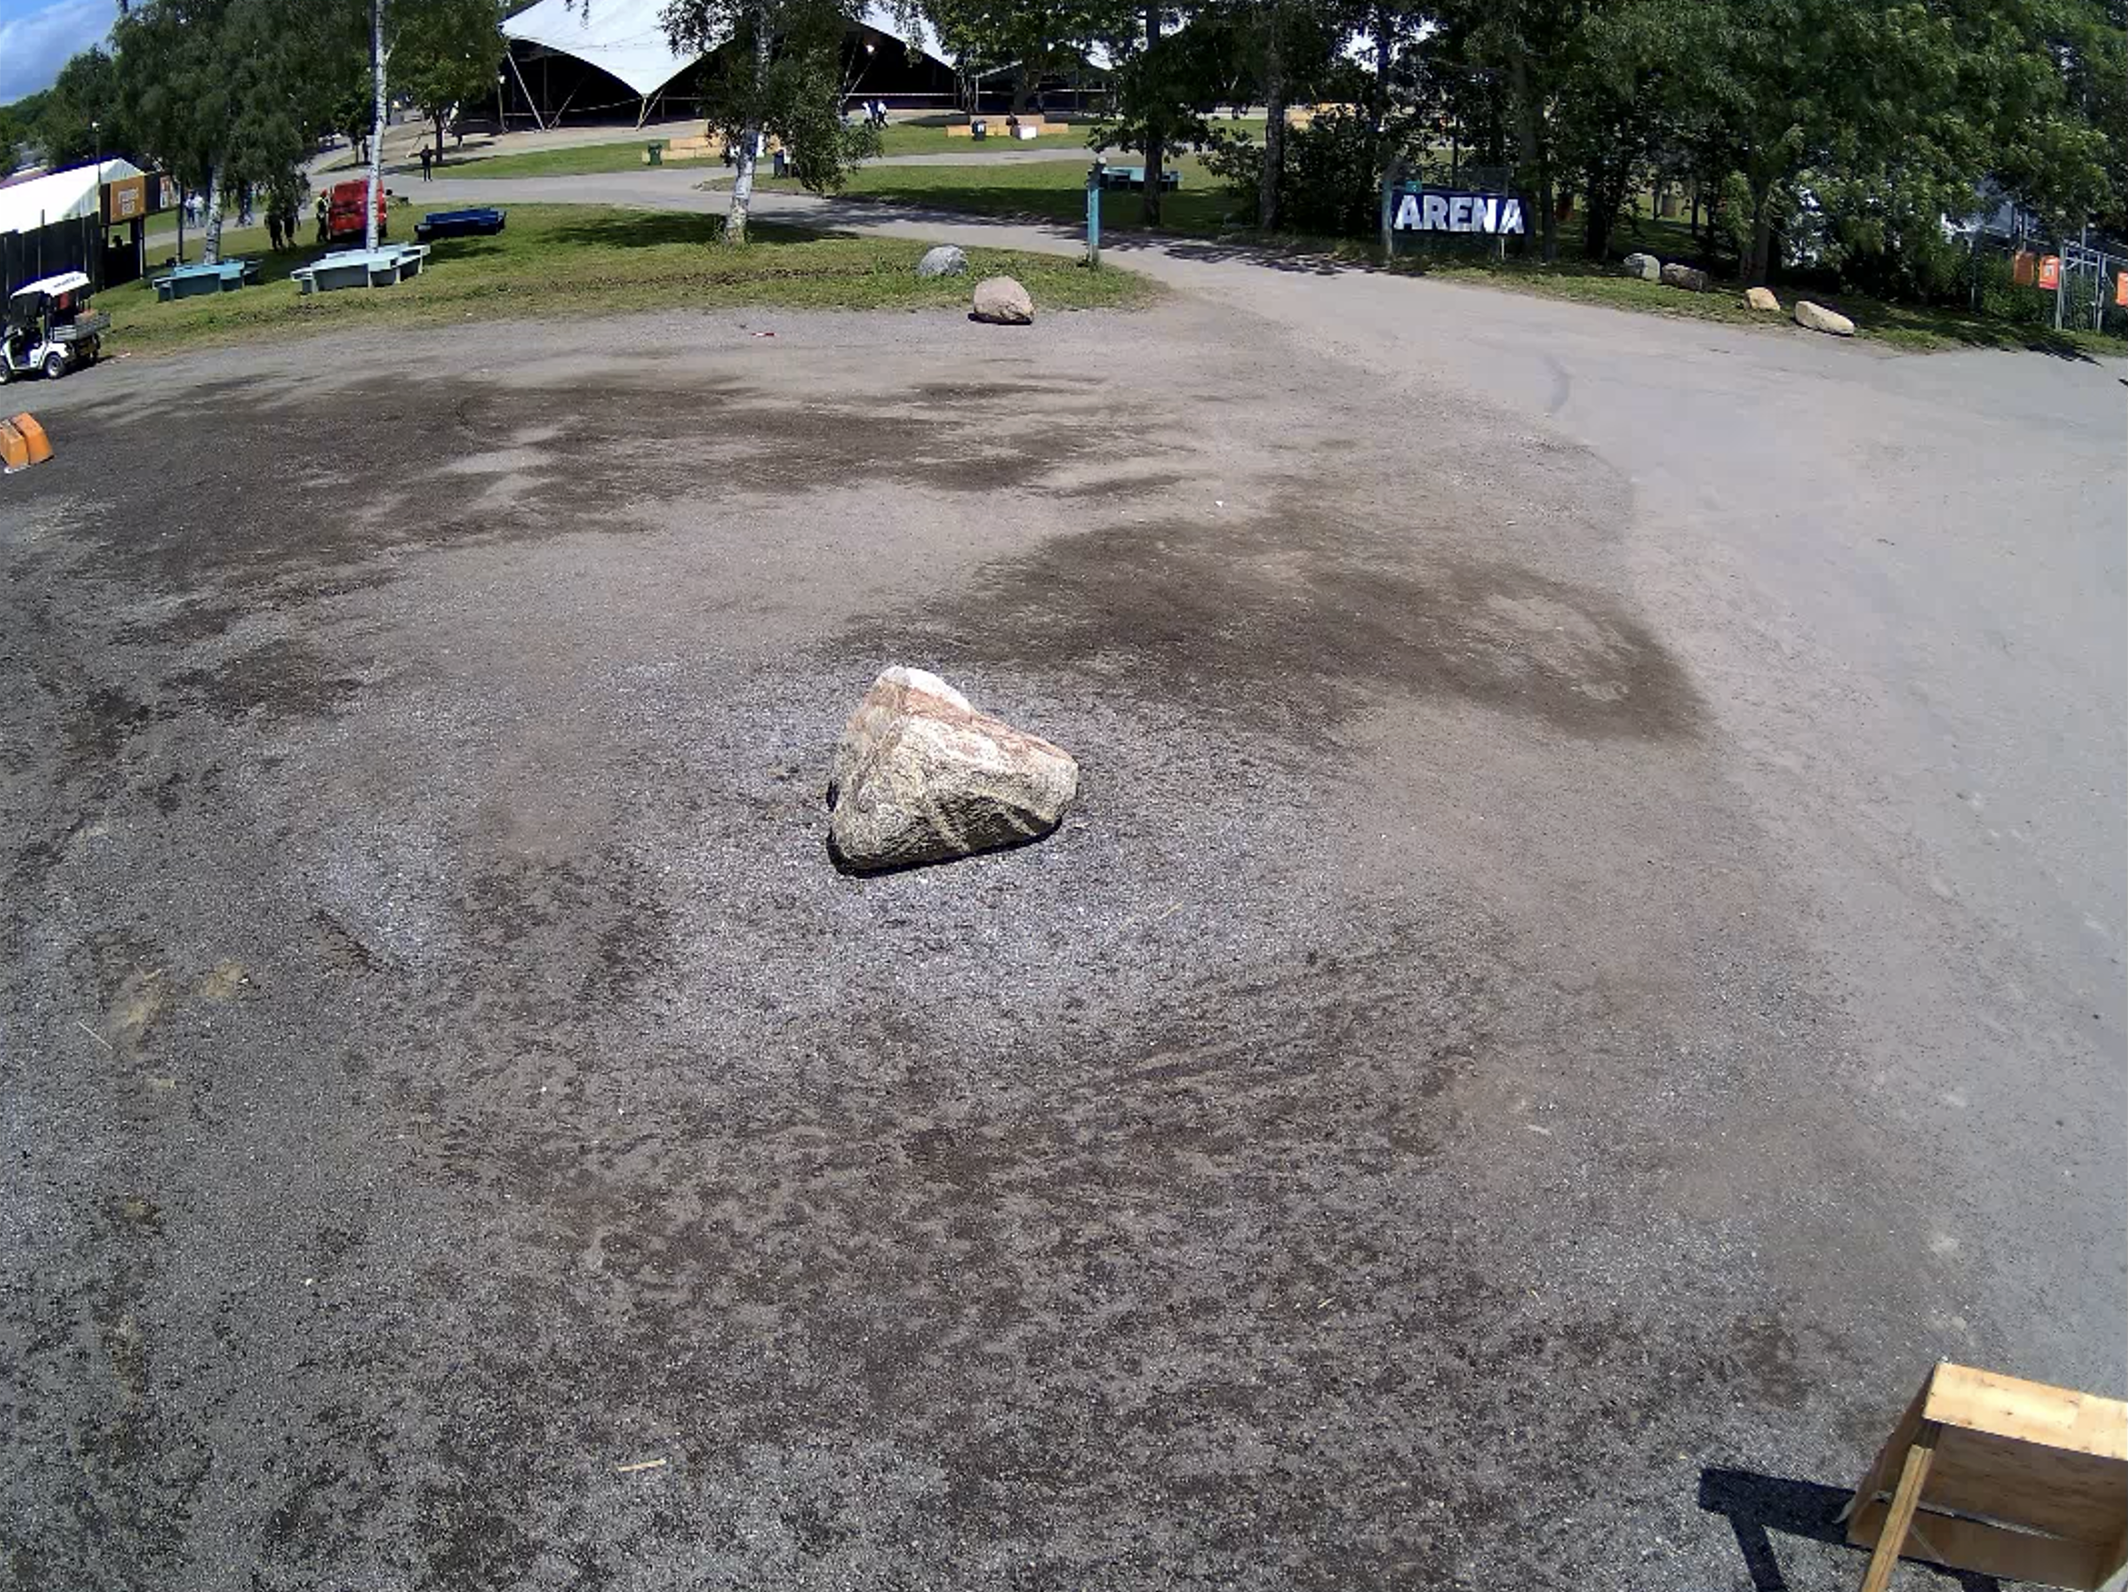
\includegraphics[width=\textwidth]{Pictures/Misc/Cameras/ARENA_CAM3.png}
    \caption{CAM3 Preview}
  \end{subfigure}%
  \hspace{0.06\textwidth}
  \begin{subfigure}{0.37\textwidth}
    \centering
    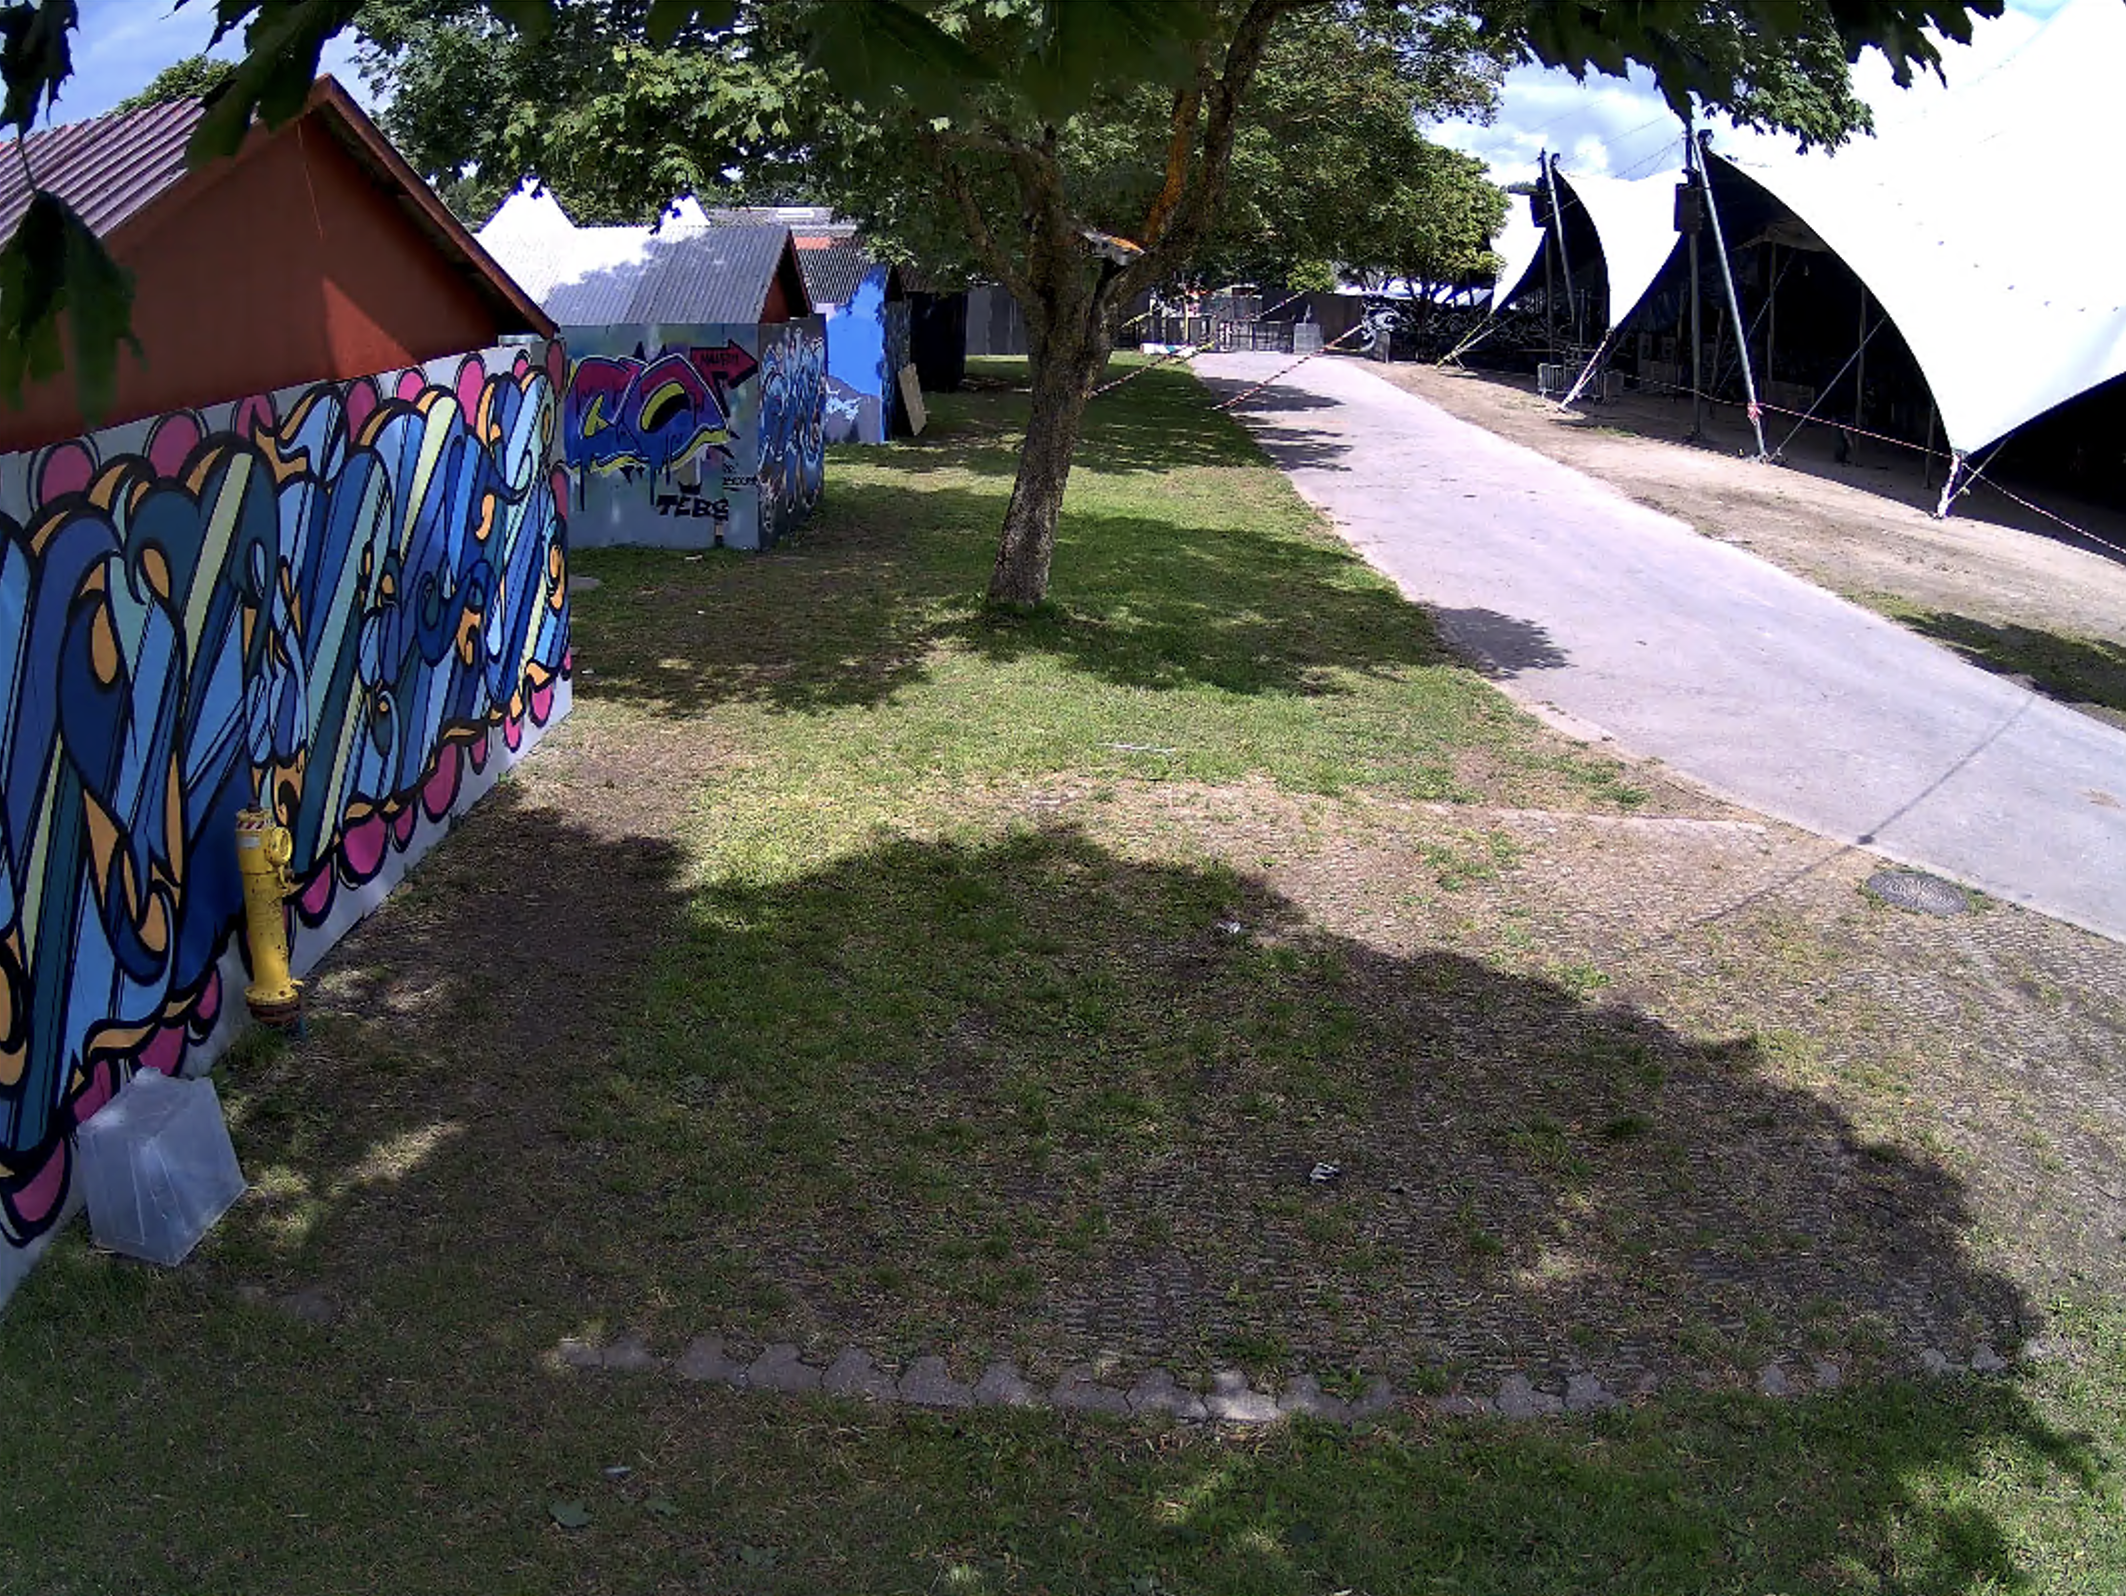
\includegraphics[width=\textwidth]{Pictures/Misc/Cameras/ARENA_CAM4.png}
    \caption{CAM4 Preview}
  \end{subfigure}

  \caption{Camera placement at Arena stage, with approximate field of view (FOV) indicated (a). The bottom images show sample frames from the four cameras deployed at the Arena stage, showing the field of view for each camera position (b-e).}
  \label{fig:arena_cameras}

\end{figure}


% 
\subsection{Computer vision model}
\label{sec:cv_model}

% - YOLOv8 (Ultralytics)
% - trained on frames annotated from each camera
% - Each camera trained separately, and weights used seperately
% - 1 class (person)
% - 1280x1280 input size

The core of the system's ability to analyze crowd dynamics relies on a robust computer vision model capable of detecting individuals within the video footage. This section details the model selection, training process, as well as its implementation for inference.

\subsubsection{Model selection}

The primary objective of the computer vision model in this system is the detection and localization of individuals within video frames; both are prerequisites for subsequent tracking and the metric extraction. Therefore, the selected model must provide image coordinates for each detected person, rather than merely an aggregate count. Methodologies in crowd analysis typically follow either density estimation approaches, which generate maps representing crowd concentration, or detection/localization-based approaches, which identify the coordinates of each individual, often via points or bounding boxes. As tracking individual trajectories is fundamental to this project's goals, localization-based methods were deemed most relevant.

The model selection process involved evaluating architectures benchmarked on an established crowd analysis dataset, NWPU-Crowd \cite{nwpu}. Other prominent datasets known for their complexity include ShanghaiTech and JHU-CROWD++ \cite{shanghai_tech} \cite{jhu_crowd}. These datasets encompass diverse scenarios and significant variations in crowd density.

One candidate architecture considered was CrowdHat, a recently proposed model aimed at enhancing the localization performance of standard object detectors within crowded environments \cite{crowdhat}. Given its high position on the NWPU-Crowd localization leaderboard as well as its availability as open-source software, CrowdHat was selected for initial evaluation.

Another prominent architecture evaluated was You Only Look Once (YOLO), representing a widely adopted family of object detectors known for high inference speed \cite{yolo}. This project employed the YOLOv8 implementation by Ultralytics. Standard YOLOv8 models are pre-trained on the large-scale COCO dataset, providing a generalized object detection capability \cite{ultralytics} \cite{coco}. However, achieving optimal performance for the specific domain of festival crowds necessitates fine-tuning this pre-trained model on representative video data captured during the event. YOLOv8 was chosen for comprehensive testing and ultimate deployment due to its established performance benchmarks, the ease of implementation offered by the Ultralytics library, as well as its significant advantage in processing speed.

% TODO
A comparison of processing efficiency revealed that CrowdHat processes frames at an average of [Insert CrowdHat Inference Time] ms/frame, whereas YOLOv8 achieves an average inference time of [Insert YOLOv8 Inference Time] ms/frame on the identical hardware configuration. Considering the practical requirement for efficient video analysis alongside robust detection accuracy, YOLOv8 offered a superior balance. Consequently, the fine-tuned YOLOv8 model was selected as the definitive detector for integration into the system.



\subsubsection{Annotation}

While pre-training on large, diverse datasets like COCO provides the YOLOv8 model with a robust general object detection capability, achieving optimal performance necessitates fine-tuning on a custom-annotated dataset. The rationale for this extends beyond simply adapting to the general festival environment; the goal is to develop highly specialized models optimized for the precise conditions and appearance characteristics encountered by each camera at each specific deployment position. It is hypothesized that such hyper-specialization yields superior detection accuracy compared to a more generalized model.

\begin{figure}
  \centering
  \includegraphics[width=\textwidth]{Pictures/Figures/annotation_flowchart.png}
  \caption{Flowchart visualizing the annotation process. \textit{Images have been intentionally blurred to protect privacy}.}
\end{figure}

% TODO: add accuracy comparison of generalized crowdhat vs specialized yolo

The annotation process utilized Label Studio, an open-source data labeling tool \cite{label_studio}. A self-hosted instance was employed to ensure data privacy and control, preventing the need to upload potentially sensitive video material captured on-site to third-party services.

Random frames were extracted from the video recordings detailed in Section \ref{sec:data_collection}. The annotation target was specifically the heads of individuals, rather than full bodies. This choice was predicated on the assumption that in dense crowd scenarios, heads are more consistently visible than entire bodies, providing a more reliable feature for detection and subsequent tracking. Bounding boxes were drawn around each identifiable head, assigned the single class label "person".

Specific annotation guidelines were established to ensure consistency:
\begin{itemize}
  \item Bounding boxes were drawn tightly around the visible extent of the head, explicitly including hair.
  \item In cases of occlusion, where one head partially blocks the view of another, overlapping bounding boxes were permitted.
  \item If individuals were distant (e.g., in the far background) or within extremely dense parts of the crowd, making distinct heads difficult to discern, bounding boxes were only placed where a head could be clearly distinguished. Ambiguous cases were omitted to maintain label quality.
\end{itemize}



To minimize time spent annotating, an iterative approach was used. After an initial batch of frames was annotated, a YOLOv8 model was trained on this preliminary data. This temporary model was then integrated with Label Studio to pre-annotate subsequent frames by suggesting bounding boxes based on its predictions. This workflow is commonly referred to as human-in-the-loop, and significantly expedited annotation time, as the task increasingly involved refining or validating the model's suggestions rather than manually creating annotations. Additionally, this methodology offered a visual indicator of model performance, as the diminishing need for manual adjustments indicated that the model was becoming more robust and that enough data had been annotated for final training.

The annotation results are summarized in Table \ref{tab:annotation_stats}.

\begin{table}
  \centering
  \label{tab:annotation_stats}
  \renewcommand{\arraystretch}{1.15}
  \begin{tabularx}{0.9\textwidth}{@{} ll >{\centering\arraybackslash}X >{\centering\arraybackslash}X @{}}
    \toprule
    Stage                                 & Camera       & Images        & Bounding Boxes \\
    \midrule
    \multirow{4}{*}{Eos}                  & CAM1         & N/A           & N/A            \\
                                          & CAM2         & 46            & 5297           \\
                                          & CAM3         & N/A           & N/A            \\
                                          & CAM4         & 18            & 1933           \\
    \midrule
    \multirow{4}{*}{Arena}                & CAM1         & 22            & 2480           \\
                                          & CAM2         & 32            & 1269           \\
                                          & CAM3         & 26            & 2075           \\
                                          & CAM4         & N/A           & N/A            \\
    \midrule \midrule
    \multicolumn{2}{@{}l}{\textbf{Total}} & \textbf{144} & \textbf{8774}                  \\
    \bottomrule
  \end{tabularx}
  \caption{Annotation statistics per camera deployment. Note that \textit{CAM1} and \textit{CAM3} at Eos stage were not annotated, as they were redundant to \textit{CAM2} and \textit{CAM4} respectively. \textit{CAM4} at Arena stage was also not annotated due to time constraints.}

  \renewcommand{\arraystretch}{1.0}
\end{table}

\subsubsection{Training}
To develop the specialized models required for each camera deployment, the YOLOv8m model, pre-trained on the COCO dataset, was fine-tuned using the custom annotated dataset (detailed in previous section). This process utilized the Ultralytics framework \cite{ultralytics}.

Training was configured with the following key hyperparameters: an input image size of 1280x1280 pixels, a batch size of 4, and training duration of 600 epochs with early stopping patience of 200 epochs. The process was optimized for the single "person" class. To accelerate the computationally intensive training process, computations were performed on a personal computer equipped with an Nvidia RTX 4080 SUPER graphics card, leveraging GPU acceleration.

This fine-tuning stage produced specialized model weights adapted to the unique visual characteristics of each camera view at the festival, which were then used for the subsequent inference stage.

\subsubsection{Inference and Tracking}
Following the training phase, the inference stage employs the specialized YOLOv8 models to detect heads within the recorded video footage, which are then tracked across frames using an object tracking algorithm. This combined inference and tracking pipeline generates the foundational data required for subsequent spatial mapping and metric extraction. The process begins by loading the fine-tuned model weights specific to the camera view being analyzed. Input videos are processed in parallel, analyzing each frame individually to identify and track individuals present. Videos are processed at a rate of 15 frames per second (FPS), which is half the recorded frame rate of 30 FPS.

Each frame is resized to a 1280x1280 pixel resolution, as defined during training, before running inference. This prepared frame is then passed to the fitted YOLOv8 model, which outputs bounding boxes around predicted heads and assigns confidence scores to these detections. These predictions are filtered; detections falling below a predefined confidence threshold are discarded (40\%), and Non-Maximum Suppression (NMS) is applied to resolve significant overlaps between bounding boxes, preserving only the most confident prediction.

The resulting bounding boxes and confidence scores are subsequently passed as input to the object tracking module. This project utilizes ByteTrack, a high-performance algorithm chosen for its accuracy, particularly within crowded scenes \cite{bytetrack}. ByteTrack associates the current frame's detections with previous frames, assigning a unique ID to each tracked individual.

The final output for each frame is a list containing the bounding box coordinates, the assigned tracking ID, and the detection confidence score for every tracked individual. This data serves as input for the spatial mapping system described in the following section.

\subsection{Spatial mapping and GIS}
\label{sec:spatial_mapping}

While the computer vision model (Section \ref{sec:cv_model}) outputs the locations of individuals in terms of pixel coordinates within the video frame, these coordinates alone are insufficient for thorough analysis of crowd dynamics. In order to derive area-based metrics such as crowd density (people per square meter), movement speeds and distances, it is necessary to translate these pixel positions into real-world geographic coordinates. Spatial mapping has this purpose, providing the planar transformation between the camera's perspective and the geographic context of the festival. This mapping also enables visualization of individual positions, from multiple cameras, onto a single overhead map, significantly enhancing contextual understanding, compared to that which is achievable through video footage alone.

The technique employed for this spatial mapping is \textit{homography}: a transformation that maps points from one plane to another. In this context, it establishes a mathematical translation between the pixel coordinates in the 2D camera image plane and the corresponding real-world coordinates on the ground plane \cite{homography}. This allows any detected pixel coordinate within a defined area to be projected onto its actual geographic location.

Performing the homography calculation requires two sets of corresponding points: one set in the camera's pixel coordinates and another in real-world coordinates. The latter is obtained from Roskilde Festival's internal Geographic Information System (GIS) tooling, which provides precise GPS coordinates of all infrastructure on the festival grounds. Selecting corresponding points was achieved by identifying distinct, stationary landmarks visible in the video frame, such as corners of structures or fences, and marking their position in pixel coordinates. These landmarks were then located in the GIS utility, where their GPS coordinates were recorded. Given a minimum of four distinct pairs of corresponding points, the homography transformation can be computed -- in this case, utilizing the OpenCV Python library \cite{opencv}. This resulting transformation is stored in a configuration file associated with that camera deployment. This manual process was performed once for each camera deployment, and the resulting homography matrices were used for all subsequent video footage captured by that camera. See Figure \ref{fig:homography_mapping} for an illustration of the results of this mapping process.

Note a slight limitation of homography in this context; homography assumes that the mapping occurs between two planar surfaces. While the surfaces in the camera and map are treated as planar, the Earth's surface is curved. For the relatively small geographic areas covered by individual camera views, the ground surface can be reasonably approximated as flat. The error introduced by this assumption is considered negligible for the purposes of crowd analysis at this scale.

\begin{figure}
  \begin{subfigure}{0.46\textwidth}
    \centering
    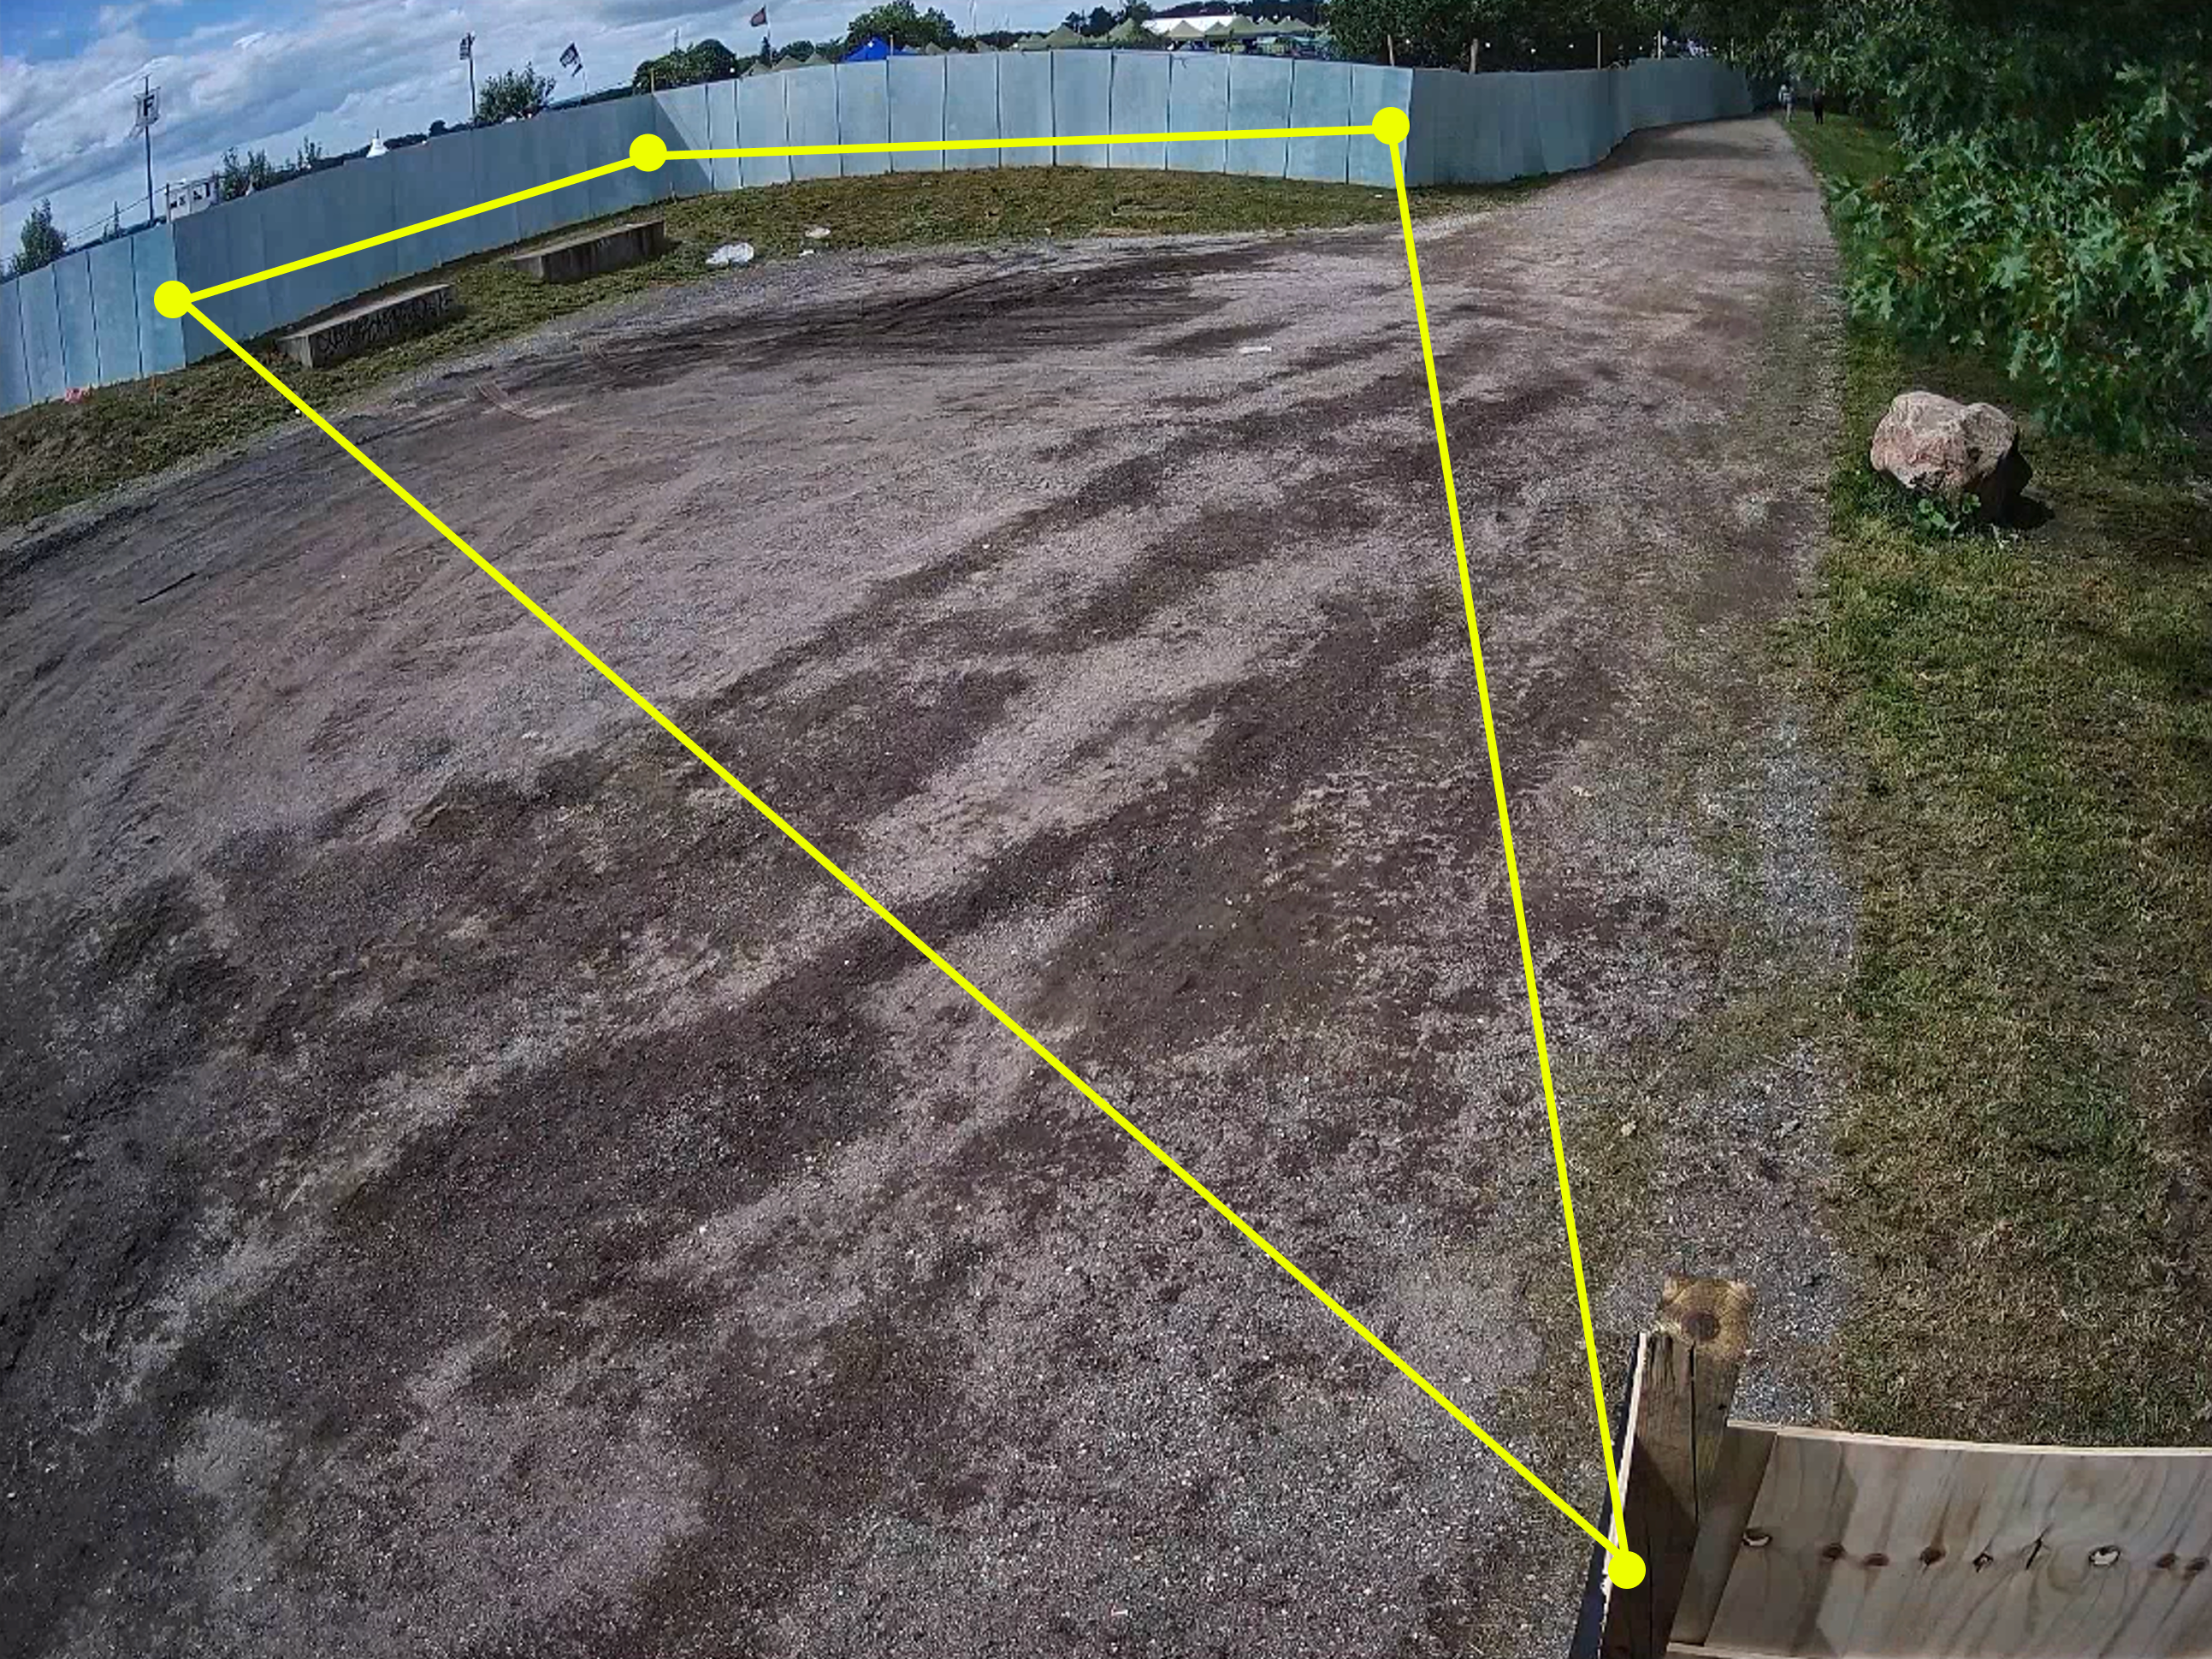
\includegraphics[width=\textwidth]{Pictures/Figures/homography_cam.png}
    \caption{Camera view}
  \end{subfigure}%
  \hspace{0.06\textwidth}
  \begin{subfigure}{0.46\textwidth}
    \centering
    \includegraphics[width=\textwidth]{Pictures/Figures/homography_map.png}
    \caption{Map view}
  \end{subfigure}
  \caption{Illustration of homography mapping between camera view and map view.}
  \label{fig:homography_mapping}
\end{figure}


\subsection{Metric extraction}
\label{sec:metric_extraction}

Following the spatial mapping process (Section \ref{sec:spatial_mapping}), which translates tracked individuals' pixel coordinates into real-world geographic coordinates, the metric extraction system processes this positional data to derive quantitative insights into crowd dynamics. This stage is the crucial step transforming raw data into the key metrics utilized by crowd safety professionals. The primary metrics extracted, as defined in Section \ref{sec:key-metrics}, include ingress/egress counts, flow rates, cumulative counts, crowd density, and movement patterns.

\subsubsection{Ingress/Egress and Flow Rate Calculation}

To measure the flow of people into and out of specific areas, lines are drawn across each camera view. These lines correspond to the entrances/exits covered by the cameras (as detailed in Section \ref{sec:data_collection}, Figures \ref{fig:eos_cameras} and \ref{fig:arena_cameras}). The system follows the trajectory of each tracked individual (identified by a unique ID from the tracking algorithm, Section \ref{sec:cv_model}). When a trajectory crosses the virtual line, the system registers it as either an ingress or egress event based on the direction of crossing.

These individual crossing events are then aggregated over specific time intervals. Intervals of 1 minute, 15 minutes, and 1 hour were identified as most useful by Roskilde Festival (Appendix \ref{appendix:rf-feb-25}). This aggregation allows the calculation of the ingress/egress flow rate, representing the number of people entering/exiting the area per time unit. The net flow rate is calculated as the difference between ingress and egress flow rates, indicating the rate of change in the number of people within the area.

Furthermore, a cumulative count provides a running total of the net number of people within the monitored area over time, calculated by aggregating ingress/egress over time. This cumulative count is particularly useful for understanding the overall occupancy of the area. These flow metrics can be calculated for individual entrances or cameras, or they can be aggregated to provide a total flow for a larger area such as an entire stage. The system also identifies and records maximum ingress and egress flow rates observed during specific periods, like during a concert. This data is essential for understanding peak loads, capacity planning, and validating entrance width calculations.

\subsubsection{Crowd Density Calculation}
Crowd density, measured in people per square meter (people/m²), is another critical metric for assessing safety and comfort. To calculate density, the monitored area is divided into a grid of 3x3 meter cells. At discrete time intervals, the system counts the number of tracked individuals whose mapped geographic coordinates (Section \ref{sec:spatial_mapping}) fall within each grid cell. The density for that cell or zone is then calculated by dividing this count by the known area of the cell or zone.

\subsubsection{Movement Patterns}

Beyond counts and density calculations, understanding how crowds move is crucial. By analyzing the sequence of time-stamped geographic coordinates, or trajectories, associated with each unique tracking ID, the system can visualize movement patterns. This involves plotting the paths taken by individuals over time, represented as gradient lines on the map.

Analyzing these patterns can reveal dominant flow directions, identifying the primary paths people take when moving between locations. It can also aid in detecting cross-flow, areas where different streams of people intersect. Additionally, this analysis helps understand origin-destination patterns, showing where people come from when approaching an area, such as which pathway they used, and where they head afterwards.


\subsection{Interface/frontend}
\label{sec:frontend}

The interface/frontend is the final component of the system, and is the only component visible to the end-users. It is therefore designed to condense the complexity of the sub-systems described in the previous sections into an accessible and user-friendly interface. The application employs a modern web development stack: namely, React, Next.js, TypeScript, and Tailwind CSS.

Data storage and retrieval is managed through a PostgreSQL database, accessed via the Prisma Object-Relational Mapper (ORM). The database contains predefined information, including camera configurations, processed count data, and timestamped geographic point data. Additionally, the database stores user login information, as well as user-generated labels/notes for specific time intervals and cameras.

The entire frontend application is deployed and hosted using Vercel. See full overview of the frontend application in Section \ref{sec:frontend-showcase}.
